\chapter{Counting the Zeros}\label{ch:counting-zeros}

\begin{chapterintro}
In Chapter~\ref{ch:zeta} you met the nontrivial zeros of the Riemann zeta function, the points $\rho_n=\tfrac12+it_n$ on the critical line. Their heights $t_n$ look irregular: $14.13$, $21.02$, $25.01$, $30.42$, \dots, with no evident rule taking you from one to the next. Suppose someone hands you these numbers one at a time. Could you say in advance, roughly, where the next one will be? Surprisingly, yes. The individual heights are hard to predict, but their \emph{average density} is known exactly. A smooth, explicit function of $t$ tells you how many zeros lie below any height, with an error that stays small: at the heights in this book it is a fraction of a zero.

This chapter derives that function. We count zeros with a tool from complex analysis, the argument principle, which turns ``how many zeros are inside this region?'' into ``how many times does the phase of the function wind around?''. Applied to the zeta function, it gives the Riemann--von Mangoldt formula $N(T)=\theta(T)/\pi+1+S(T)$. Stirling's formula (Chapter~\ref{ch:asymptotics}) then turns $\theta(T)$ into an elementary expression, and out drops the smooth counting function with its curious constant $\tfrac78$. From it we build the ``smooth zeros'' $s_n$, the local mean spacing $\gap_n$, and the idea of measuring every error in units of that spacing.

\textbf{Where this shows up in the paper.} The smooth counting function is the paper's Eq.~(1); the smooth zeros and mean spacing are defined in its Sec.~II~A; and every rms number in every table of the paper (Tables I--V) is in units of $\gap_n$. The principal ``null'' error $0.263$, against which the models in the paper are judged on its principal holdout, is simply the rms size of the fluctuation $(t_n-s_n)/\gap_n$ over zeros 401--500, a quantity you will compute yourself at the end of this chapter.
\end{chapterintro}

\begin{prerequisites}
\item Chapter~\ref{ch:complex}: complex numbers in polar form, modulus and argument, the argument of a product is the sum of the arguments, $a^s=e^{s\log a}$, the logarithm of a complex number and its branches.
\item Chapter~\ref{ch:series}: the series $\log(1+y)=y-\tfrac{y^2}{2}+\dots$ for $\abs{y}<1$, the geometric series, alternating series and their sums.
\item Chapter~\ref{ch:asymptotics}: big-$\order$ notation; Stirling's formula for $\log\Gamma$, including the complex form stated there; inverting a monotone function; bisection, Newton and Brent root finding; the Lambert $W$ function.
\item Chapter~\ref{ch:zeta}: $\zeta(s)$, the Euler product and the fact that $\zeta(s)\neq0$ for $\Re s>1$; the alternating zeta $\eta(s)=(1-2^{1-s})\zeta(s)$; the pole at $s=1$; trivial zeros; the critical strip and line; the functional equation (stated there); the Riemann--Siegel $Z$ function; computing zeros with \texttt{mpmath.zetazero}.
\item First-year physics and calculus: derivatives, the chain rule, Taylor expansion to second order, and reading a graph.
\end{prerequisites}

%=====================================================================
\section{The staircase $N(T)$}\label{sec:counting-zeros-staircase}
% DYK-BEGIN
\begin{didyouknow}{Fifteen Zeros by Hand}
In 1903 the Danish mathematician J{\o}rgen Gram computed the first fifteen nontrivial zeros of zeta and confirmed that they lie on the critical line. The first sits at height $t\approx14.1347$. Gram points, where a related phase passes a multiple of $\pi$, are still used to count zeros efficiently. They usually, but not always, alternate with the zeros.
\end{didyouknow}
% DYK-END

\subsection{Definition}

Recall from Chapter~\ref{ch:zeta} that a nontrivial zero of $\zeta$ is written $\rho_n=\tfrac12+it_n$ with $t_n>0$ its \emph{height} (strictly, the imaginary part of the zero; writing the real part as $\tfrac12$ assumes the zero is on the critical line, which has been verified numerically for every zero used in this book). The zeros with negative imaginary part are mirror images of these, so we only ever count the upper half.

\begin{quote}
\textbf{Definition.} For $T>0$, the \emph{zero-counting function} $N(T)$ is the number of nontrivial zeros $\rho$ of $\zeta$ with $0<\Im\rho\le T$, each counted as many times as its multiplicity.
\end{quote}

``Multiplicity'' means this: if $\zeta$ vanished like $(s-\rho)^2$ near $\rho$ we would count $\rho$ twice. Every zero ever computed has turned out to be simple (multiplicity one). That is a \emph{numerical observation}; nobody has proved that all zeros are simple.

$N(T)$ is a staircase. It is zero for $T<t_1$, jumps to 1 at $t_1$, stays flat until $t_2$, jumps to 2, and so on. Our running example RE1 lists the first ten heights:
\begin{multline}
t_1,\dots,t_{10}=14.134725,\ 21.022040,\ 25.010858,\ 30.424876,\ 32.935062,\\
37.586178,\ 40.918719,\ 43.327073,\ 48.005151,\ 49.773832.
\label{eq:counting-zeros-RE1}
\end{multline}

\begin{sample}{Reading the staircase}
Using RE1, find $N(30)$, $N(40)$ and $N(50)$, and find the average spacing of the first ten zeros.

\textbf{Step 1:} $N(30)$ counts heights $\le30$. From the list, $t_1,t_2,t_3$ are below 30 and $t_4=30.42>30$. So $N(30)=3$.

\textbf{Step 2:} For $T=40$: $t_6=37.59<40<t_7=40.92$, so $N(40)=6$.

\textbf{Step 3:} For $T=50$: $t_{10}=49.77<50$, and the next zero (not in the list) is above 50, as you can confirm with \texttt{mpmath.zetazero(11)}, whose imaginary part is $52.97$. So $N(50)=10$.

\textbf{Step 4:} The average spacing of the first ten zeros is the total distance divided by the number of gaps:
\[
\frac{t_{10}-t_1}{9}=\frac{49.773832-14.134725}{9}=\frac{35.639107}{9}=3.9599.
\]

\[
\boxed{N(30)=3,\quad N(40)=6,\quad N(50)=10,\quad \text{mean spacing of } t_1,\dots,t_{10}\approx 3.96.}
\]
\end{sample}

Ten zeros between heights 14 and 50 give spacings of about 4. If you look higher up, at zeros near number 1000, the spacing is closer to 1. The zeros crowd together as you go up. We want a formula that captures this crowding exactly.

\subsection{The smooth curve through the staircase}

Figure~\ref{fig:counting-zeros-staircase} shows $N(T)$ up to $T=100$ together with the smooth function
\begin{equation}
\Nsm(t)=\frac{t}{2\pi}\log\frac{t}{2\pi}-\frac{t}{2\pi}+\frac78,
\label{eq:counting-zeros-Nsm}
\end{equation}
which is the paper's Eq.~(1). Throughout, $\log$ is the natural logarithm. The smooth curve threads through the staircase, passing close to the middle of each vertical riser. The whole purpose of Secs.~\ref{sec:counting-zeros-winding}--\ref{sec:counting-zeros-theta} is to derive Eq.~\eqref{eq:counting-zeros-Nsm} and to say exactly what the difference $N(T)-\Nsm(T)$ is.

\begin{figure}[htbp]\centering
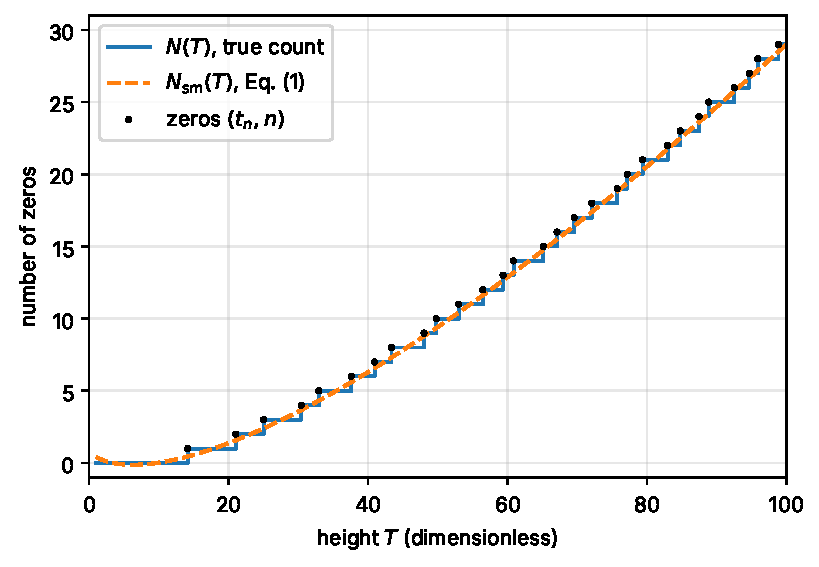
\includegraphics[width=0.85\linewidth]{figs/counting-zeros_staircase.pdf}
\caption{The zero-counting function $N(T)$ (staircase) for $0<T\le100$ and the smooth counting function $\Nsm(T)$ of Eq.~\eqref{eq:counting-zeros-Nsm} (dashed). Dots mark the zeros $t_n$ at height $n$. The smooth curve passes near the midpoint of each riser; at $T=100$ it gives $29.002$ while $N(100)=29$.}
\label{fig:counting-zeros-staircase}
\end{figure}

\begin{sample}{Evaluating the smooth count}
Evaluate $\Nsm(50)$ and compare with $N(50)=10$.

\textbf{Step 1:} Compute $t/2\pi$. With $2\pi=6.283185$, $50/2\pi=7.957747$.

\textbf{Step 2:} Its logarithm is easiest as a difference: $\log(50/2\pi)=\log50-\log(2\pi)=3.912023-1.837877=2.074146$.

\textbf{Step 3:} First term: $7.957747\times2.074146=16.505529$.

\textbf{Step 4:} Subtract $t/2\pi$ and add $7/8$:
\[
\Nsm(50)=16.505529-7.957747+0.875=9.422782.
\]

\textbf{Step 5:} Compare: $N(50)-\Nsm(50)=10-9.4228=0.5772$.

\[
\boxed{\Nsm(50)\approx 9.423,\qquad N(50)-\Nsm(50)\approx 0.577.}
\]
The smooth formula is off by about half a zero at this height, even though nothing in it ``knows'' where the individual zeros are.
\end{sample}

The same arithmetic gives $\Nsm(30)=3.565$ against $N(30)=3$, $\Nsm(40)=6.293$ against $N(40)=6$, and $\Nsm(100)=29.002$ against $N(100)=29$. The difference wanders up and down but stays well below 1. Those differences are the subject of Sec.~\ref{sec:counting-zeros-S}.

\begin{pycode}
import numpy as np, qmnt
t = qmnt.zeros(100)                 # heights t_1 ... t_100
def N(T):                           # number of zeros with 0 < t_n <= T
    return np.searchsorted(t, T, side="right")
def Nsm(T):                         # paper Eq. (1)
    u = T/(2*np.pi)
    return u*np.log(u) - u + 7/8
for T in [30, 40, 50, 100]:
    print(T, N(T), round(Nsm(T), 4), round(N(T) - Nsm(T), 4))
\end{pycode}

\subsection{Why a smooth curve should cross $n-\tfrac12$ at the $n$-th zero}

A staircase that jumps from $n-1$ to $n$ at $t_n$ has, at that point, a riser running from height $n-1$ to height $n$. A smooth curve that ``averages'' the staircase should cut each riser near its middle, at height $n-\tfrac12$. This suggests a natural smooth stand-in for the $n$-th zero: the height $s_n$ at which the smooth curve reaches $n-\tfrac12$. We return to this definition in Sec.~\ref{sec:counting-zeros-smooth}. For the same reason we introduce, for a simple zero, the \emph{midpoint value} of the staircase at $t_n$:
\[
N^{\rm mid}(t_n)=\tfrac12\bigl[N(t_n^-)+N(t_n^+)\bigr]=\tfrac12\bigl[(n-1)+n\bigr]=n-\tfrac12,
\]
the average of the value just below the zero ($n-1$) and the value just above it ($n$). This is a separate symbol: by the definition of $N(T)$, which includes $T$ itself, $N(t_n)=n$.

\begin{checkpoint}
Is $N(T)$ a continuous function of $T$? By how much does it jump at a zero of multiplicity 2?
\checkanswer{No. It is constant between zeros and jumps at each zero. At a zero of multiplicity 2 it jumps by 2, because each zero is counted with its multiplicity. (No such zero is known.)}
\end{checkpoint}

\begin{keyideas}
\item $N(T)$ counts the zeros with $0<t_n\le T$; it is a staircase.
\item The zeros crowd together with height: spacings near 4 at the bottom, near 1 around zero 1000.
\item The smooth function $\Nsm(t)$ of Eq.~\eqref{eq:counting-zeros-Nsm} threads the staircase, crossing each riser near its midpoint $n-\tfrac12$.
\end{keyideas}

%=====================================================================
\section{Counting by winding: the argument principle}\label{sec:counting-zeros-winding}

How could one count zeros of a function without finding them? For real functions of a real variable you count sign changes. For complex functions there is a much more powerful idea: walk around a closed loop and watch the \emph{phase} of the function.

\subsection{Following the argument continuously}

Recall from Chapter~\ref{ch:complex} that any nonzero complex number $w$ can be written $w=\abs{w}e^{i\arg w}$, where the argument $\arg w$ is defined only up to adding multiples of $2\pi$. Now let $z$ move along a path $C$ in the complex plane, and suppose $f(z)\neq0$ everywhere on $C$. As $z$ moves, the point $f(z)$ moves, and we can choose values of $\arg f(z)$ that change \emph{continuously}, never jumping by $2\pi$. (Picture following a runner on a circular track and counting laps rather than reporting only the compass direction.) The \emph{net change of the argument along $C$} is
\begin{equation}
\Delta_C\arg f=\bigl(\text{final value of }\arg f\bigr)-\bigl(\text{initial value of }\arg f\bigr),
\label{eq:counting-zeros-deltaarg}
\end{equation}
computed with this continuous choice. It does not depend on which value we start with, because changing the start by $2\pi k$ changes the finish by the same $2\pi k$.

\subsection{One factor at a time}

Take the simplest function with a zero, $f(z)=z-a$, and let $C$ be a circle traversed once counterclockwise.

\emph{Case 1: $a$ inside the circle.} First suppose the circle is centered at $a$: $z=a+re^{i\phi}$, $0\le\phi\le2\pi$. Then $f(z)=re^{i\phi}$, whose argument is $\phi$ itself, so $\Delta_C\arg f=2\pi$. If the circle is not centered at $a$ but still encloses it, a geometric argument settles the matter (look at the left panel of Fig.~\ref{fig:counting-zeros-winding}). A disk is convex, so every ray leaving the interior point $a$ crosses the circle exactly once. Hence, as $z$ goes once round the circle, the direction of $z-a$ takes every compass direction exactly once. It can never turn back, because turning back would make it take some direction twice. So it turns steadily the same way through one full turn, and the net change is again $2\pi$.

\emph{Case 2: $a$ outside the circle.} Draw the two tangent lines from $a$ to the circle. The whole circle lies inside the wedge between them, and the opening angle of that wedge is less than $\pi$. The direction of $z-a$ therefore always stays inside a range of angles narrower than $\pi$. A continuously followed argument that never leaves such a range cannot gain a full turn, so it returns to its starting value: $\Delta_C\arg f=0$. (Both cases are geometric arguments for circles; the general theorem is stated below.)

Now take a product $f(z)=(z-a_1)(z-a_2)\cdots(z-a_k)$. From Chapter~\ref{ch:complex}, the argument of a product is the sum of the arguments of the factors. Therefore the net change of $\arg f$ around $C$ is the sum of the net changes of the factors: $2\pi$ for every $a_j$ inside $C$ and $0$ for every $a_j$ outside. Dividing by $2\pi$:
\begin{equation}
\frac{1}{2\pi}\Delta_C\arg f=\text{number of zeros of }f\text{ inside }C.
\label{eq:counting-zeros-argprinciple}
\end{equation}
A zero repeated twice, $(z-a)^2$, contributes $2\times2\pi$, so the count includes multiplicity automatically.

\begin{sample}{Winding of a cubic}
Let $f(z)=(z-1)(z-2)(z+3)$ and let $C$ be the circle $\abs{z}=2.5$ traversed counterclockwise. Predict $\Delta_C\arg f/2\pi$ and confirm it numerically.

\textbf{Step 1:} Locate the zeros: $z=1$, $z=2$, $z=-3$. Their distances from the origin are $1$, $2$ and $3$.

\textbf{Step 2:} The circle has radius $2.5$, so $1$ and $2$ are inside and $-3$ is outside.

\textbf{Step 3:} By Eq.~\eqref{eq:counting-zeros-argprinciple}, the factors $z-1$ and $z-2$ each contribute $2\pi$, and $z+3$ contributes 0. So $\Delta_C\arg f=4\pi$.

\textbf{Step 4 (numerical check):} Sample $z=2.5e^{i\phi}$ at many values of $\phi$, compute the argument of $f$ at each, remove the artificial $2\pi$ jumps (\texttt{np.unwrap}), and take last minus first. The listing below prints $2.0000$ for the ratio.

\[
\boxed{\frac{1}{2\pi}\Delta_C\arg f=2.}
\]
\end{sample}

\begin{pycode}
import numpy as np
phi = np.linspace(0, 2*np.pi, 20001)     # one counterclockwise turn
z = 2.5*np.exp(1j*phi)
f = (z - 1)*(z - 2)*(z + 3)
ph = np.unwrap(np.angle(f))              # continuous argument
print((ph[-1] - ph[0])/(2*np.pi))        # number of enclosed zeros
\end{pycode}

\begin{figure}[htbp]\centering
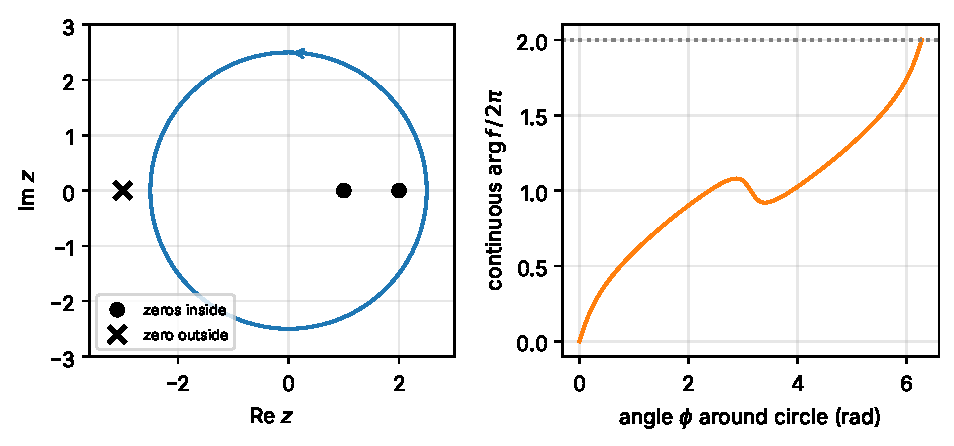
\includegraphics[width=0.85\linewidth]{figs/counting-zeros_winding.pdf}
\caption{The argument principle for $f(z)=(z-1)(z-2)(z+3)$. Left: the circle $\abs{z}=2.5$ (traversed counterclockwise) and the three zeros; two lie inside. Right: the continuously followed argument of $f$ along the circle, divided by $2\pi$, against the angle $\phi$ around the circle. It rises by exactly 2 over one turn, the number of enclosed zeros.}
\label{fig:counting-zeros-winding}
\end{figure}

\begin{pitfall}
\texttt{np.angle} returns the \emph{principal} argument, in $(-\pi,\pi]$. Each time the true argument passes $\pi$ the principal value jumps down by $2\pi$. If you subtract first from last principal values you always get something in $(-2\pi,2\pi)$, which hides the winding. Always apply \texttt{np.unwrap} (which adds back the $2\pi$ jumps) and sample the path finely enough that the true argument changes by much less than $\pi$ between samples.
\end{pitfall}

\subsection{The general theorem}

Most functions are not polynomials, so we cannot factor them into finitely many $(z-a_j)$. The intuition still holds. An \emph{analytic} function (one that has a complex derivative at every point of a region) behaves near each zero like a constant times $(z-a)^k$, with $k$ a positive integer; this local form is itself part of what we take on trust below. Away from its zeros its argument can be followed continuously inside the region without net winding. Making this precise is a theorem of complex analysis that we take on trust.

\begin{beyond}
\textbf{The argument principle (proved; proof beyond this book).} Let $f$ be analytic (complex-differentiable) at every point inside and on a simple closed curve $C$, traversed counterclockwise, and suppose $f$ has no zeros on $C$. Then the number of zeros of $f$ inside $C$, counted with multiplicity, equals $\frac{1}{2\pi}\Delta_C\arg f$. The proof uses contour integration of $f'/f$ (the residue theorem). See the chapter on complex variables in \cite{rhb}.
\end{beyond}

Two requirements of the theorem matter below: $f$ must be analytic everywhere inside and on $C$ (no poles), and $f$ must not vanish on $C$ itself (otherwise the argument is undefined there).

\begin{checkpoint}
You walk around a circle that encloses no zero of an analytic function $f$. What is $\Delta_C\arg f$? What goes wrong if the circle passes exactly through a zero?
\checkanswer{The net change is $0$. If the circle passes through a zero, $f=0$ there and its argument is undefined, so the count is not defined; the theorem excludes this case.}
\end{checkpoint}

\begin{keyideas}
\item Following the phase of $f$ continuously around a closed loop and dividing the net change by $2\pi$ counts the zeros inside, with multiplicity.
\item For products, phases add, so each enclosed zero contributes one full turn.
\item The general argument principle requires $f$ analytic inside and on the loop and nonzero on the loop.
\end{keyideas}

%=====================================================================
\section{The Riemann--von Mangoldt formula}\label{sec:counting-zeros-rvm}

We now apply the argument principle to count the zeros of $\zeta$ in a tall rectangle. There is one obstacle: $\zeta$ has a pole at $s=1$ and trivial zeros at $s=-2,-4,\dots$, and the theorem needs a function analytic everywhere inside the loop whose zeros are exactly the ones we want. Riemann's remedy is to multiply $\zeta$ by factors that cancel the pole and the trivial zeros.

\subsection{The completed zeta function}

Define
\begin{equation}
\xi(s)=\tfrac12\,s(s-1)\,\pi^{-s/2}\,\Gamma\!\left(\tfrac s2\right)\zeta(s),
\label{eq:counting-zeros-xi}
\end{equation}
where $\Gamma$ is the gamma function (the generalized factorial of Chapter~\ref{ch:asymptotics}) and $\pi^{-s/2}=e^{-(s/2)\log\pi}$ as in Chapter~\ref{ch:complex}. The properties we need are collected here.

\begin{beyond}
\textbf{Properties of $\xi$ (proved; proofs beyond this book; see \cite{edwards}, Chs.~1--2, or \cite{titchmarsh}, Ch.~2).}
\begin{itemize}
\item[(a)] $\xi$ extends to a function analytic at every point of the complex plane. The pole of $\zeta$ at $s=1$ is canceled by the factor $s-1$; the poles of $\Gamma(s/2)$ at $s=0,-2,-4,\dots$ are canceled by the factor $s$ (at $s=0$) and by the trivial zeros of $\zeta$ (at $s=-2,-4,\dots$).
\item[(b)] Functional equation in symmetric form: $\xi(s)=\xi(1-s)$. (This is the functional equation of Chapter~\ref{ch:zeta} rewritten.)
\item[(c)] Reflection: $\xi(\bar s)=\overline{\xi(s)}$, because $\xi$ is real on the real axis.
\item[(d)] $\Gamma(z)$ is never zero, and $\Gamma(x)>0$ for real $x>0$.
\item[(e)] $\zeta(s)\neq0$ for $\Re s\ge1$. (For $\Re s>1$ this follows from the Euler product, Chapter~\ref{ch:zeta}; on the line $\Re s=1$ it is a deeper theorem, closely tied to the prime number theorem.)
\end{itemize}
Consequences: the zeros of $\xi$ are exactly the nontrivial zeros of $\zeta$, all in the strip $0<\Re s<1$. Indeed, by (a), (d) and (e), none of the factors in Eq.~\eqref{eq:counting-zeros-xi} vanishes for $\Re s\ge1$ except $s-1$ at $s=1$, where it cancels the pole of $\zeta$ and leaves $\xi(1)=\tfrac12\neq0$ (shown below); by (b), $\xi$ has no zeros with $\Re s\le0$ either; inside the strip the extra factors are nonzero, so $\xi$ vanishes exactly where $\zeta$ does, with the same multiplicity.
\end{beyond}

One more property we can prove ourselves, using only Chapter~\ref{ch:zeta}.

\textbf{Claim:} $\xi(\sigma)>0$ for every real $\sigma$ with $-1\le\sigma\le2$.

\emph{Proof.} Split into ranges.
\begin{enumerate}
\item $1<\sigma\le2$. Here the constant $\tfrac12$ is positive, $\zeta(\sigma)=\sum_k k^{-\sigma}>0$ (a sum of positive terms), $\sigma(\sigma-1)>0$, $\pi^{-\sigma/2}>0$ and $\Gamma(\sigma/2)>0$ by (d). The product of these five positive numbers is positive.
\item $0<\sigma<1$. Recall $\eta(\sigma)=1-2^{-\sigma}+3^{-\sigma}-4^{-\sigma}+\cdots$, an alternating series whose terms decrease in size (because $\sigma>0$, $k^{-\sigma}$ decreases as $k$ increases) and tend to zero. From Chapter~\ref{ch:series}, its sum lies between any two consecutive partial sums, in particular between $1-2^{-\sigma}$ and $1$. Since $2^{-\sigma}<1$, the sum satisfies $\eta(\sigma)\ge1-2^{-\sigma}>0$. Also $1-2^{1-\sigma}<0$ because $1-\sigma>0$ makes $2^{1-\sigma}>1$. Hence $\zeta(\sigma)=\eta(\sigma)/(1-2^{1-\sigma})<0$. Meanwhile $\sigma(\sigma-1)<0$ (positive times negative). In Eq.~\eqref{eq:counting-zeros-xi} the two negative factors multiply to a positive number, and the remaining factors are positive, so $\xi(\sigma)>0$.
\item $\sigma=1$ and $\sigma=0$. Near $s=1$, $(s-1)\zeta(s)\to1$ (the pole has residue 1, Chapter~\ref{ch:zeta}), and $\Gamma(\tfrac12)=\sqrt\pi$, so $\xi(1)=\tfrac12\cdot1\cdot\pi^{-1/2}\cdot\sqrt\pi\cdot1=\tfrac12>0$. By (b), $\xi(0)=\xi(1)=\tfrac12$.
\item $-1\le\sigma<0$. By (b), $\xi(\sigma)=\xi(1-\sigma)$, and $1-\sigma$ lies in $(1,2]$, where we showed $\xi>0$. $\square$
\end{enumerate}

\subsection{The contour}

Fix a height $T>0$ that is \emph{not} the height of any zero. Let $R$ be the rectangle with corners $-1$, $2$, $2+iT$, $-1+iT$ (Fig.~\ref{fig:counting-zeros-contour}), traversed counterclockwise. Check the conditions of the argument principle for $f=\xi$:
\begin{itemize}
\item $\xi$ is analytic everywhere, by (a).
\item No zeros on the bottom edge (the real segment $[-1,2]$): we just proved $\xi>0$ there.
\item No zeros on the right edge $\Re s=2$ or the left edge $\Re s=-1$: all zeros of $\xi$ have $0<\Re s<1$.
\item No zeros on the top edge $\Im s=T$: we chose $T$ not to be the height of a zero.
\end{itemize}
Inside $R$ the zeros of $\xi$ are the nontrivial zeros with $0<\Im\rho<T$; there are $N(T)$ of them. So
\begin{equation}
N(T)=\frac{1}{2\pi}\Delta_{\partial R}\arg\xi,
\label{eq:counting-zeros-NR}
\end{equation}
where $\partial R$ denotes the boundary of $R$ traversed counterclockwise.

\begin{figure}[htbp]\centering
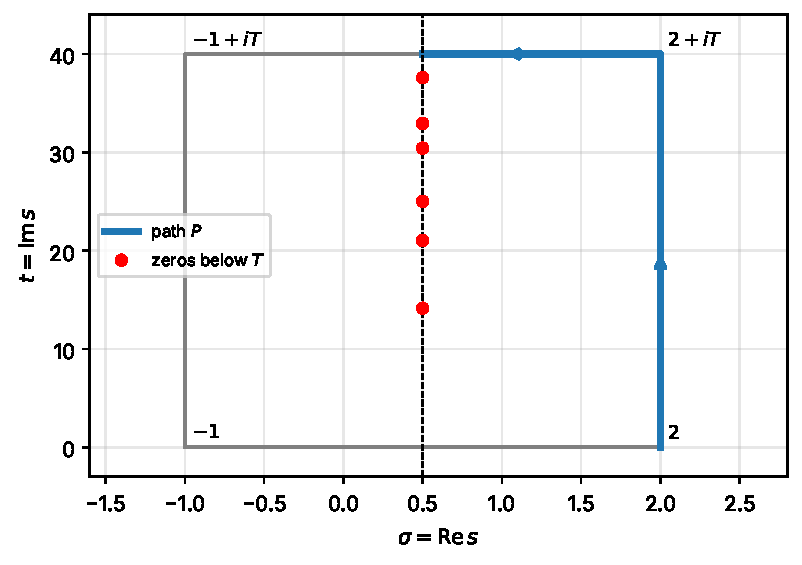
\includegraphics[width=0.85\linewidth]{figs/counting-zeros_contour.pdf}
\caption{The contour used to count zeros of $\xi$ up to height $T=40$. The rectangle has corners $-1$, $2$, $2+iT$ and $-1+iT$ in the complex $s$-plane ($\sigma=\Re s$, $t=\Im s$). Dots: the six zeros $\tfrac12+it_n$ below height 40. The thick path $P$ runs from $2$ up to $2+iT$ and left to $\tfrac12+iT$; by symmetry, the change of $\arg\xi$ around the whole rectangle is twice its change along $P$. The dashed line is the critical line $\sigma=\tfrac12$.}
\label{fig:counting-zeros-contour}
\end{figure}

\subsection{Halving the contour by symmetry}

Split $\partial R$ into three pieces:
\begin{enumerate}
\item the bottom edge, from $-1$ to $2$;
\item the right half $P$: from $2$ up to $2+iT$, then left to $\tfrac12+iT$;
\item the left half $P'$: from $\tfrac12+iT$ left to $-1+iT$, then down to $-1$.
\end{enumerate}
(The top edge is split at $\tfrac12+iT$ between $P$ and $P'$.)

\emph{Bottom edge.} There $\xi$ is real and positive, so its argument can be taken to be $0$ all along. The net change is $0$.

\emph{Left half.} Consider the map $s\mapsto s^*=1-\bar s$, which reflects a point across the critical line $\Re s=\tfrac12$ (it sends $\sigma+it$ to $(1-\sigma)+it$). Combining properties (b) and (c):
\begin{equation}
\xi(1-\bar s)=\xi(\bar s)=\overline{\xi(s)}.
\label{eq:counting-zeros-reflect}
\end{equation}
The first equality is (b) applied at the point $\bar s$; the second is (c). Now the reflection sends $2\mapsto-1$, $2+iT\mapsto-1+iT$ and $\tfrac12+iT\mapsto\tfrac12+iT$. So $P'$, which runs $\tfrac12+iT\to-1+iT\to-1$, is the mirror image of $P$ run backwards ($\tfrac12+iT\to2+iT\to2$). Two things happen to the argument:
\begin{itemize}
\item Running $P$ backwards reverses the sign of the net change: $-\Delta_P\arg\xi$.
\item By Eq.~\eqref{eq:counting-zeros-reflect}, the values of $\xi$ on $P'$ are the complex conjugates of the values at the mirror points, and conjugation negates the argument. This reverses the sign again.
\end{itemize}
The two sign reversals cancel: $\Delta_{P'}\arg\xi=+\Delta_P\arg\xi$. Adding the three pieces,
\begin{equation}
\Delta_{\partial R}\arg\xi=0+\Delta_P\arg\xi+\Delta_{P'}\arg\xi=2\,\Delta_P\arg\xi,
\end{equation}
and Eq.~\eqref{eq:counting-zeros-NR} becomes
\begin{equation}
N(T)=\frac{1}{\pi}\Delta_P\arg\xi.
\label{eq:counting-zeros-NP}
\end{equation}

\subsection{Factor by factor}

Since $\xi$ is a product, $\Delta_P\arg\xi$ is the sum of the changes of the arguments of the factors in Eq.~\eqref{eq:counting-zeros-xi} (Chapter~\ref{ch:complex}). We take them one at a time along $P$, which starts at $s=2$ and ends at $s=\tfrac12+iT$.

\emph{The constant $\tfrac12$.} Its argument is always 0: change $0$.

\emph{The factor $s(s-1)$.} At the start, $s=2$ and $s-1=1$ are both positive reals, with argument 0. Along the vertical part of $P$, both $s$ and $s-1$ have positive real part, so their arguments stay in $(-\pi/2,\pi/2)$ without jumps. Along the horizontal part, the imaginary part is fixed at $T>0$, so the arguments of $s$ and $s-1$ stay in $(0,\pi)$, again without jumps. At the end:
\begin{align*}
\arg s&=\arg\!\left(\tfrac12+iT\right)=\arctan(2T),\\
\arg(s-1)&=\arg\!\left(-\tfrac12+iT\right)=\pi-\arctan(2T),
\end{align*}
where the second line uses that $-\tfrac12+iT$ is the mirror image of $\tfrac12+iT$ across the imaginary axis. Adding, the change of $\arg[s(s-1)]$ is
\begin{equation}
\arctan(2T)+\pi-\arctan(2T)=\pi.
\end{equation}

\emph{The factor $\pi^{-s/2}$.} With $s=\sigma+it$, $\pi^{-s/2}=e^{-(\sigma/2)\log\pi}\,e^{-i(t/2)\log\pi}$. The first factor is a positive real number; the second has argument $-(t/2)\log\pi$. This argument is $0$ at $s=2$ and $-(T/2)\log\pi$ at the end. Change: $-\tfrac T2\log\pi$.

\emph{The factor $\Gamma(s/2)$.} As $s$ runs along $P$, $s/2$ runs from $1$ to $1+iT/2$ to $\tfrac14+iT/2$, always in the right half-plane $\Re z>0$, where $\Gamma$ is analytic and never zero. At the start $\Gamma(1)=1$, argument 0. The change is therefore $\arg\Gamma(\tfrac14+\tfrac{iT}2)$, where the argument is followed continuously from $\Gamma(1)$. Equivalently, it is $\Im\log\Gamma(\tfrac14+\tfrac{iT}{2})$, where $\log\Gamma$ is the branch of the logarithm that is real on the positive real axis and continuous in the right half-plane. (Because $\Gamma$ has no zeros in the right half-plane, any path from $1$ to $\tfrac14+iT/2$ inside it gives the same continuous argument; this is the branch used by Stirling's formula in Sec.~\ref{sec:counting-zeros-theta}.)

\emph{The factor $\zeta(s)$.} We give its change a name. Along $P$, $\zeta$ does not vanish: on $\Re s=2$ by the Euler product, and on the top edge because $T$ is not the height of a zero. At the start $\zeta(2)=\pi^2/6>0$, argument 0.

\begin{quote}
\textbf{Definitions.} The \emph{Riemann--Siegel theta function} is
\begin{equation}
\theta(T)=\Im\log\Gamma\!\left(\tfrac14+\tfrac{iT}{2}\right)-\frac T2\log\pi,
\label{eq:counting-zeros-thetadef}
\end{equation}
with the continuous branch just described (so $\theta(0)=0$). The function $S(T)$ is
\begin{equation}
S(T)=\frac1\pi\Delta_P\arg\zeta=\frac1\pi\arg\zeta\!\left(\tfrac12+iT\right),
\label{eq:counting-zeros-Sdef}
\end{equation}
where $\arg\zeta(\tfrac12+iT)$ means the value reached by continuous variation along $P$, starting from $\arg\zeta(2)=0$.
\end{quote}

The factors $\tfrac12$, $s(s-1)$, $\pi^{-s/2}$ and $\Gamma(s/2)$ together contribute $0+\pi-\tfrac T2\log\pi+\Im\log\Gamma(\tfrac14+\tfrac{iT}2)=\pi+\theta(T)$, and $\zeta$ contributes $\pi S(T)$. Insert into Eq.~\eqref{eq:counting-zeros-NP}:
\begin{equation}
N(T)=\frac1\pi\bigl[\pi+\theta(T)+\pi S(T)\bigr]
\quad\Longrightarrow\quad
\boxed{N(T)=\frac{\theta(T)}{\pi}+1+S(T)}
\label{eq:counting-zeros-RvM}
\end{equation}
for every $T>0$ that is not the height of a zero. This is the \textbf{Riemann--von Mangoldt formula}. Riemann stated the leading behavior in 1859 \cite{riemann1859}; von Mangoldt gave the first complete proof decades later \cite{edwards,titchmarsh}. Its status in this book: a theorem. The proof above is complete modulo the results taken on trust in the boxes: the argument principle, and properties (a)--(e) of $\xi$ and $\Gamma$ (of which (e) on the line $\Re s=1$ is a deep theorem).

Notice what we have achieved. The left side counts zeros, which are hard to find. On the right, $\theta(T)$ is a property of the gamma function, which we understand very well, and all the difficulty is pushed into $S(T)$, the argument of $\zeta$ on the critical line.

\begin{checkpoint}
Why does the formula require that $T$ not be the height of a zero? Name the step of the derivation that fails.
\checkanswer{If $T=t_n$, then $\xi$ (and $\zeta$) vanish at a point of the top edge of the rectangle, so $\arg\xi$ is undefined there and the argument principle does not apply. Equivalently, $S(T)$ in Eq.~\eqref{eq:counting-zeros-Sdef} is undefined at $T=t_n$.}
\end{checkpoint}

\begin{keyideas}
\item $\xi(s)$ removes the pole and trivial zeros of $\zeta$ and is symmetric under $s\to1-s$; its zeros are exactly the nontrivial zeros.
\item Counting zeros of $\xi$ in a rectangle with the argument principle, and halving by symmetry, gives $N(T)=\theta(T)/\pi+1+S(T)$, Eq.~\eqref{eq:counting-zeros-RvM}.
\item The $+1$ comes from the factor $s(s-1)$, whose argument changes by $\pi$; $\theta$ comes from $\pi^{-s/2}\Gamma(s/2)$; $S$ comes from $\zeta$ itself.
\end{keyideas}

%=====================================================================
\section{The theta function and the constant $\tfrac78$}\label{sec:counting-zeros-theta}

\subsection{Stirling's formula for complex argument}

Recall from Chapter~\ref{ch:asymptotics} Stirling's formula, stated there for complex argument:

\begin{beyond}
\textbf{Stirling's formula (proved; proof beyond this book; see \cite{rhb}, or any text on the gamma function).} As $\abs z\to\infty$ with $\abs{\arg z}\le\pi-\delta$ for some fixed $\delta>0$,
\begin{equation}
\log\Gamma(z)=\left(z-\tfrac12\right)\log z-z+\tfrac12\log(2\pi)+\frac{1}{12z}+\order\!\left(\abs z^{-3}\right),
\label{eq:counting-zeros-stirling}
\end{equation}
where $\log z$ is the principal logarithm and $\log\Gamma$ is the branch real on the positive real axis.
\end{beyond}

We apply it with $z=\tfrac14+\tfrac{it}{2}$, $t>0$ large. Then $\abs z\approx t/2$ is large and $\arg z$ is close to $\pi/2$, safely inside the allowed range.

\subsection{Derivation of the asymptotic formula for $\theta$}

We need $\Im\log\Gamma(z)$, term by term. Throughout, $t>0$.

\textbf{Step A: modulus of $z$.} 
\begin{equation}
\abs z^2=\frac1{16}+\frac{t^2}{4}=\frac{t^2}{4}\left(1+\frac1{4t^2}\right).
\end{equation}
Taking logarithms and halving,
\begin{equation}
\log\abs z=\log\frac t2+\frac12\log\!\left(1+\frac{1}{4t^2}\right).
\end{equation}
Using $\log(1+y)=y-\tfrac{y^2}{2}+\cdots$ with $y=1/(4t^2)$ (Chapter~\ref{ch:series}),
\begin{equation}
\log\abs z=\log\frac t2+\frac{1}{8t^2}+\order(t^{-4}).
\label{eq:counting-zeros-logmod}
\end{equation}

\textbf{Step B: argument of $z$.} Since $\Re z=\tfrac14>0$, $\arg z=\arctan\!\bigl(\Im z/\Re z\bigr)=\arctan(2t)$. For $a>0$, if $\varphi=\arctan a\in(0,\pi/2)$ then $\tan(\pi/2-\varphi)=\cot\varphi=1/a$, so $\arctan a=\pi/2-\arctan(1/a)$. Hence
\begin{equation}
\arg z=\frac\pi2-\arctan\frac{1}{2t}.
\end{equation}
For small $y$, $\arctan y=y-\tfrac{y^3}{3}+\cdots$: this follows by integrating $\frac{\dd}{\dd y}\arctan y=\frac1{1+y^2}=1-y^2+y^4-\cdots$ (a geometric series in $-y^2$, Chapter~\ref{ch:series}) term by term from $0$. With $y=1/(2t)$,
\begin{equation}
\arg z=\frac\pi2-\frac{1}{2t}+\order(t^{-3}).
\label{eq:counting-zeros-argz}
\end{equation}

\textbf{Step C: the term $(z-\tfrac12)\log z$.} Write $z-\tfrac12=-\tfrac14+\tfrac{it}{2}$ and $\log z=\log\abs z+i\arg z$. For two complex numbers $(a+ib)(c+id)$ the imaginary part is $ad+bc$. Here $a=-\tfrac14$, $b=\tfrac t2$, $c=\log\abs z$, $d=\arg z$:
\begin{equation}
\Im\!\left[\left(z-\tfrac12\right)\log z\right]=-\frac14\arg z+\frac t2\log\abs z.
\end{equation}
Substitute Eqs.~\eqref{eq:counting-zeros-logmod} and \eqref{eq:counting-zeros-argz}:
\begin{align}
\frac t2\log\abs z&=\frac t2\log\frac t2+\frac{1}{16t}+\order(t^{-3}),\\
-\frac14\arg z&=-\frac\pi8+\frac{1}{8t}+\order(t^{-3}).
\end{align}

\textbf{Step D: the term $-z$.} $\Im(-z)=-\dfrac t2$.

\textbf{Step E: the constant.} $\tfrac12\log(2\pi)$ is real: imaginary part $0$.

\textbf{Step F: the term $1/(12z)$.} Multiply numerator and denominator by $\bar z$: $\dfrac1z=\dfrac{\bar z}{\abs z^2}=\dfrac{\tfrac14-\tfrac{it}{2}}{\abs z^2}$. So
\begin{equation}
\Im\frac{1}{12z}=-\frac{t/2}{12\abs z^2}=-\frac{t}{24\abs z^2}=-\frac{t}{6t^2\left(1+\frac{1}{4t^2}\right)}=-\frac{1}{6t}+\order(t^{-3}),
\end{equation}
where we used $24\abs z^2=24\cdot\frac{t^2}{4}(1+\frac1{4t^2})=6t^2(1+\frac1{4t^2})$ and $1/(1+y)=1-y+\cdots$.

\textbf{Step G: the remainder.} $\order(\abs z^{-3})=\order(t^{-3})$.

\textbf{Step H: add everything.} Collecting Steps C to G,
\begin{equation}
\Im\log\Gamma\!\left(\tfrac14+\tfrac{it}{2}\right)=\frac t2\log\frac t2-\frac t2-\frac\pi8+\left(\frac1{16}+\frac18-\frac16\right)\frac1t+\order(t^{-3}).
\end{equation}
The bracket is $\frac{3}{48}+\frac{6}{48}-\frac{8}{48}=\frac{1}{48}$.

\textbf{Step I: subtract $\tfrac t2\log\pi$} (Eq.~\eqref{eq:counting-zeros-thetadef}) and combine logarithms, $\frac t2\log\frac t2-\frac t2\log\pi=\frac t2\log\frac{t}{2\pi}$:
\begin{equation}
\boxed{\theta(t)=\frac t2\log\frac{t}{2\pi}-\frac t2-\frac\pi8+\frac{1}{48t}+\order(t^{-3}).}
\label{eq:counting-zeros-thetaasym}
\end{equation}
Status: a proved asymptotic expansion (given Stirling). Carrying Stirling one term further shows that the $\order(t^{-3})$ term is $\frac{7}{5760\,t^3}$; you can confirm this coefficient numerically in Problem~23.

\subsection{Where $\tfrac78$ comes from}

Divide Eq.~\eqref{eq:counting-zeros-thetaasym} by $\pi$:
\begin{equation}
\frac{\theta(T)}{\pi}=\frac{T}{2\pi}\log\frac{T}{2\pi}-\frac{T}{2\pi}-\frac18+\frac{1}{48\pi T}+\order(T^{-3}).
\end{equation}
Add 1 and use Eq.~\eqref{eq:counting-zeros-RvM}:
\begin{equation}
N(T)=\underbrace{\frac{T}{2\pi}\log\frac{T}{2\pi}-\frac{T}{2\pi}+\frac78}_{\Nsm(T)}+S(T)+\frac{1}{48\pi T}+\order(T^{-3}).
\label{eq:counting-zeros-NsmS}
\end{equation}
The constant is $-\tfrac18+1=\tfrac78$: the $-\tfrac18$ is the $-\pi/8$ of Stirling divided by $\pi$, and the $+1$ is the half turn of $s(s-1)$. This is exactly the paper's Eq.~(1). The leftover $1/(48\pi T)$ is tiny: at $T=t_1=14.13$ it is $4.7\times10^{-4}$, and it shrinks further with height. So, up to an $\order(1/T)$ term,
\begin{equation}
N(T)\approx\Nsm(T)+S(T).
\label{eq:counting-zeros-split}
\end{equation}

\begin{sample}{The theta function at $T=50$}
Evaluate $\theta(50)$ from Eq.~\eqref{eq:counting-zeros-thetaasym}, compare with the exact value from \texttt{mpmath.siegeltheta}, and deduce $S(50)$ from Eq.~\eqref{eq:counting-zeros-RvM}.

\textbf{Step 1:} From the earlier Sample Problem, $\log(50/2\pi)=2.0741459$. So $\frac{50}{2}\log\frac{50}{2\pi}=25\times2.0741459=51.853648$.

\textbf{Step 2:} Subtract $\frac t2=25$: $26.853648$.

\textbf{Step 3:} Subtract $\pi/8=0.392699$: $26.460949$.

\textbf{Step 4:} Add $\frac{1}{48\times50}=\frac{1}{2400}=0.000417$: $\theta(50)\approx26.461366$. The exact value, \texttt{mpmath.siegeltheta(50)}, agrees to all digits shown; the next correction $7/(5760\times50^3)$ is about $10^{-8}$.

\textbf{Step 5:} $\theta(50)/\pi=26.461366/3.141593=8.422914$.

\textbf{Step 6:} From Eq.~\eqref{eq:counting-zeros-RvM} with $N(50)=10$: $S(50)=10-1-8.422914=0.577086$.

\[
\boxed{\theta(50)\approx26.4614,\qquad S(50)\approx+0.577.}
\]
This agrees with \texttt{mpmath.backlunds(50)}, which computes $S$ directly from the argument of $\zeta$, and with $N(50)-\Nsm(50)=0.577$ found earlier (the two differ only by $1/(48\pi\cdot50)=1.3\times10^{-4}$).
\end{sample}

\begin{pycode}
import numpy as np, mpmath as mp
def theta_asym(t):                       # Eq. (counting-zeros-thetaasym)
    return t/2*np.log(t/(2*np.pi)) - t/2 - np.pi/8 + 1/(48*t)
for t in [10.0, 30.0, 50.0]:
    exact = float(mp.siegeltheta(t))
    print(t, exact, theta_asym(t), exact - theta_asym(t))
# Riemann--von Mangoldt check: S(T) = N(T) - 1 - theta(T)/pi
print(10 - 1 - float(mp.siegeltheta(50))/np.pi, float(mp.backlunds(50)))
\end{pycode}

\begin{figure}[htbp]\centering
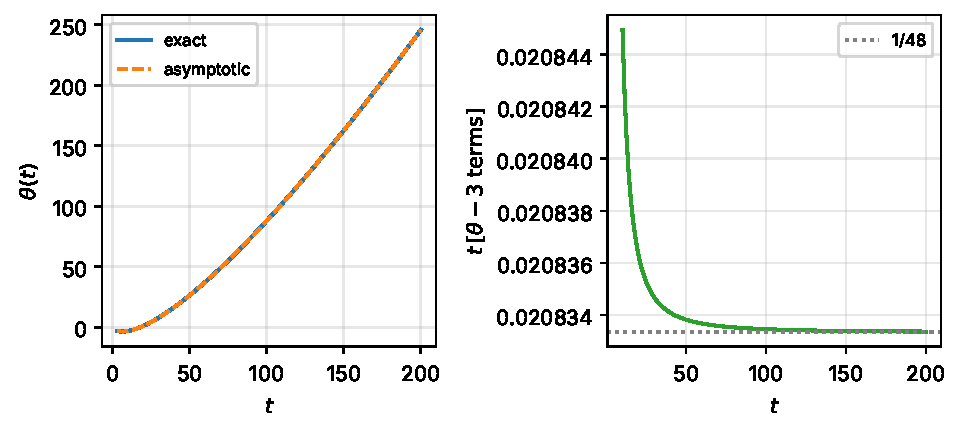
\includegraphics[width=0.85\linewidth]{figs/counting-zeros_theta.pdf}
\caption{Left: the Riemann--Siegel theta function $\theta(t)$ computed exactly with \texttt{mpmath.siegeltheta} (solid) and the asymptotic formula Eq.~\eqref{eq:counting-zeros-thetaasym} without its $\order(t^{-3})$ remainder (dashed); the two are indistinguishable except at small $t$. Right: $t$ times the difference between the exact $\theta(t)$ and the first three terms $\frac t2\log\frac t{2\pi}-\frac t2-\frac\pi8$, against $t$; it approaches $1/48$ (horizontal line), confirming the $1/(48t)$ term derived in Steps A to I. Both axes are dimensionless.}
\label{fig:counting-zeros-theta}
\end{figure}

\begin{pitfall}
Do not confuse $\theta(T)/\pi+1$ with $\Nsm(T)$. They differ by $1/(48\pi T)+\order(T^{-3})$. This book puts that tiny term into the ``fluctuating part''; the paper simply uses Eq.~(1) as its smooth part and never mentions the term. Some texts instead define the fluctuating part exactly as $S(T)$ and keep the $1/(48\pi T)$ in the smooth part. At the heights of this book the difference is below $5\times10^{-4}$ of a zero, far below every effect we study.
\end{pitfall}

\begin{checkpoint}
Where does each part of the constant $\tfrac78$ come from?
\checkanswer{$-\tfrac18$ is the $-\pi/8$ in Stirling's expansion of $\Im\log\Gamma(\tfrac14+\tfrac{iT}2)$, divided by $\pi$; it comes from $-\tfrac14\arg z$ with $\arg z\to\pi/2$. The $+1$ is the change $\pi$ in the argument of the factor $s(s-1)$ along the path, divided by $\pi$.}
\end{checkpoint}

\begin{keyideas}
\item Stirling's formula gives $\theta(t)=\frac t2\log\frac t{2\pi}-\frac t2-\frac\pi8+\frac1{48t}+\order(t^{-3})$, derived term by term in Steps A to I.
\item Hence $N(T)=\Nsm(T)+S(T)+\frac{1}{48\pi T}+\order(T^{-3})$, with $\Nsm$ the paper's Eq.~(1).
\item The constant $\tfrac78=-\tfrac18+1$ has a precise origin in the gamma factor and the factor $s(s-1)$.
\end{keyideas}

%=====================================================================
\section{The fluctuating part $S(T)$}\label{sec:counting-zeros-S}
% DYK-BEGIN
\begin{didyouknow}{The Most Slowly Growing Noise}
In 1946 Atle Selberg proved that the fluctuating part $S(T)$ of the zero count behaves statistically like a Gaussian random variable with variance about $\tfrac{1}{2\pi^2}\log\log T$. That growth is absurdly slow: even at $T=10^{20}$, $\log\log T$ is only about $3.8$. This is why $S(T)$ stays small in every computation, although it is known to be unbounded.
\end{didyouknow}
% DYK-END

\subsection{Shape of $S(T)$}

Rearranging Eq.~\eqref{eq:counting-zeros-RvM},
\begin{equation}
S(T)=N(T)-1-\frac{\theta(T)}{\pi}.
\label{eq:counting-zeros-Sfromcount}
\end{equation}
Two properties follow at once.

\emph{At a zero, $S$ jumps up.} $\theta$ is continuous, but $N$ jumps by 1 at a simple zero, so $S$ jumps by $+1$ there (by $k$ at a zero of multiplicity $k$).

\emph{Between zeros, $S$ decreases steadily.} Between consecutive zeros $N$ is constant, so
\begin{equation}
\frac{\dd S}{\dd T}=-\frac{\theta'(T)}{\pi}.
\end{equation}
Differentiating an asymptotic expansion term by term is not automatically legitimate: a small remainder can still have a large derivative. Here it is legitimate, because Stirling's expansion of $\log\Gamma(z)$ may itself be differentiated term by term in the same sector, giving the corresponding expansion of $\Gamma'(z)/\Gamma(z)$ with remainder $\order(\abs z^{-4})$; this is a proved property of the gamma function that we take on trust (it is proved in texts on the gamma function). With that understood, differentiating Eq.~\eqref{eq:counting-zeros-thetaasym} term by term (product rule on the first term: $\frac{\dd}{\dd T}\bigl[\frac T2\log\frac T{2\pi}\bigr]=\frac12\log\frac T{2\pi}+\frac T2\cdot\frac1T=\frac12\log\frac{T}{2\pi}+\frac12$),
\begin{equation}
\theta'(T)=\frac12\log\frac{T}{2\pi}+\frac12-\frac12-\frac{1}{48T^2}+\order(T^{-4})=\frac12\log\frac{T}{2\pi}-\frac{1}{48T^2}+\order(T^{-4}),
\end{equation}
so
\begin{equation}
\frac{\dd S}{\dd T}=-\frac{1}{2\pi}\log\frac{T}{2\pi}+\frac{1}{48\pi T^2}+\order(T^{-4}).
\label{eq:counting-zeros-Sslope}
\end{equation}
For $T>2\pi$ the slope is negative. So $S(T)$ is a \emph{sawtooth}: it drifts down between zeros and jumps up by 1 at each zero (Fig.~\ref{fig:counting-zeros-Sfunc}). If the zeros were perfectly evenly spaced at the local mean spacing, the downward drift between two zeros would exactly cancel each jump, and $S$ would oscillate between fixed limits. The actual irregular placement of the zeros is what makes $S$ wander.

\begin{figure}[htbp]\centering
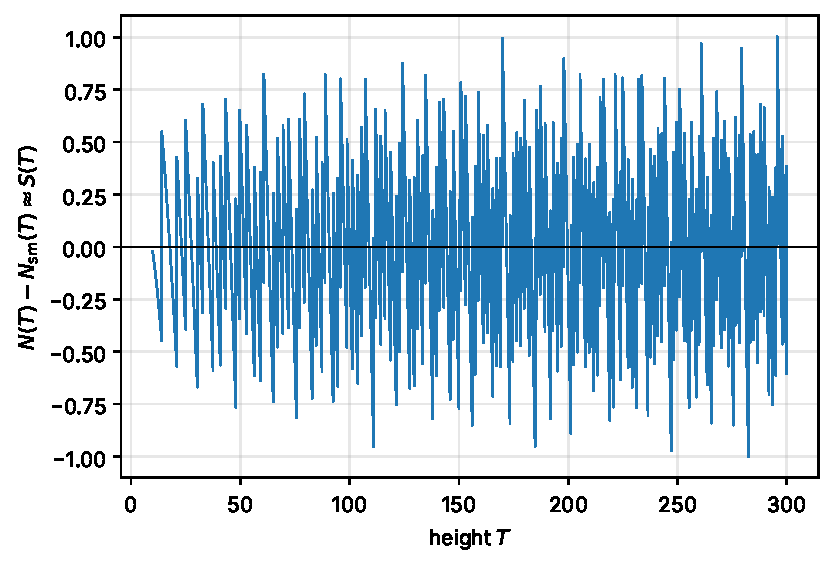
\includegraphics[width=0.85\linewidth]{figs/counting-zeros_Sfunc.pdf}
\caption{The fluctuating part $N(T)-\Nsm(T)$, which equals $S(T)$ up to the term $1/(48\pi T)$, for $10\le T\le300$ (dimensionless count against height $T$). It jumps by $+1$ at every zero and decreases between zeros with slope $-\frac{1}{2\pi}\log\frac{T}{2\pi}$. Despite the jumps, it stays within a band of width about 2 around zero over the whole range shown.}
\label{fig:counting-zeros-Sfunc}
\end{figure}

\begin{sample}{Values of $S$ at several heights}
Using $\Nsm$ and the counts $N(30)=3$, $N(40)=6$, $N(100)=29$, find $S(30)$, $S(40)$ and $S(100)$.

\textbf{Step 1:} From Eq.~\eqref{eq:counting-zeros-NsmS}, $S(T)=N(T)-\Nsm(T)-\frac1{48\pi T}$ to excellent accuracy (error $\order(T^{-3})$, below $10^{-7}$ here).

\textbf{Step 2:} $T=30$: $\log(30/2\pi)=\log30-\log2\pi=3.401197-1.837877=1.563320$. Then $\Nsm(30)=4.774648\times1.563320-4.774648+0.875=7.464305-4.774648+0.875=3.564656$. And $\frac{1}{48\pi\times30}=0.000221$. So $S(30)=3-3.564656-0.000221=-0.564877$.

\textbf{Step 3:} $T=40$: $\log(40/2\pi)=3.688879-1.837877=1.851002$; $\Nsm(40)=6.366198\times0.851002+0.875=5.417650+0.875=6.292650$. (Here we used $u\log u-u=u(\log u-1)$ with $u=T/2\pi$.) Then $S(40)=6-6.292650-0.000166=-0.292816$.

\textbf{Step 4:} $T=100$: $\log(100/2\pi)=4.605170-1.837877=2.767293$; $\Nsm(100)=15.915494\times1.767293+0.875=28.127344+0.875=29.002344$. Then $S(100)=29-29.002344-0.000066=-0.002410$.

\[
\boxed{S(30)\approx-0.565,\qquad S(40)\approx-0.293,\qquad S(100)\approx-0.002.}
\]
Each value agrees with \texttt{mpmath.backlunds} (see the CHECKS script). All three, and $S(50)=+0.577$ from the previous Sample Problem, are well below 1 in magnitude.
\end{sample}

\begin{checkpoint}
Just after a zero, is $S(T)$ larger or smaller than just before it? Between two zeros, does it increase or decrease?
\checkanswer{Larger: it jumps up by 1 at a simple zero. Between zeros it decreases, with slope $-\frac1{2\pi}\log\frac{T}{2\pi}$ (for $T>2\pi$).}
\end{checkpoint}

\subsection{How big is $S(T)$?}

The numbers above suggest that $S$ is a quantity of order a few tenths. What is known for certain is weaker but still striking.

\begin{beyond}
\textbf{Size of $S(T)$ (proved; proofs beyond this book; see \cite{titchmarsh}, Ch.~9).} (i) $S(T)=\order(\log T)$: it grows at most logarithmically. (ii) $S(T)$ is not bounded: it takes arbitrarily large positive and negative values as $T\to\infty$, but extremely slowly. (iii) Selberg proved that its mean square grows like $\frac{1}{2\pi^2}\log\log T$, so its typical size grows like $\sqrt{\log\log T}$. The function $\log\log T$ is famously sluggish: it is about $1.9$ at $T=10^3$ and about $2.2$ at $T=10^4$.
\end{beyond}

So at the heights used in the paper (up to about $t\approx 9900$, zero $10^4$) we expect $S$ to be of order a few tenths, growing only very gently with height. The paper's own numbers confirm this: the rms size of the fluctuation at the zeros (defined precisely in Sec.~\ref{sec:counting-zeros-unfold}) grows from $0.263$ on zeros 401--500 to $0.296$ on zeros 5001--10000 (paper Table~V, ``null'' column).

Historically, Backlund in 1914 used exactly this machinery to show that there are precisely 79 zeros below height 200 \cite{edwards}; you can confirm with \texttt{qmnt.zeros} that $t_{79}<200<t_{80}$.

\subsection{Counting zeros on the line: how RH is checked numerically}

Chapter~\ref{ch:zeta} introduced the Riemann--Siegel $Z$ function, $Z(t)=e^{i\theta(t)}\zeta(\tfrac12+it)$, which is real for real $t$; its $\theta$ is the same theta function as Eq.~\eqref{eq:counting-zeros-thetadef}. Because $\abs{Z(t)}=\abs{\zeta(\tfrac12+it)}$, every sign change of $Z$ between two heights marks a zero \emph{on the critical line}. Now combine two facts:
\begin{itemize}
\item Counting sign changes of $Z$ in $(0,T)$ gives a \emph{lower bound} on the number of zeros on the line below $T$ (each sign change needs at least one zero of odd multiplicity).
\item The Riemann--von Mangoldt formula gives the \emph{total} number of zeros below $T$, on or off the line, with multiplicity.
\end{itemize}
If the two numbers agree, then every zero below $T$ lies on the line and is simple: there is no room left for a zero off the line or a double zero. The catch is that Eq.~\eqref{eq:counting-zeros-RvM} needs the exact integer $N(T)$, and $S(T)$ is not given by any closed formula.

\begin{beyond}
\textbf{Turing's method (proved; details beyond this book; see \cite{edwards}, Ch.~8).} Turing showed how to determine the integer $N(T)$ rigorously from computed values of $Z$, using a bound on the average of $S(t)$ over an interval. This is the method by which RH has been verified numerically for very many zeros (Chapter~\ref{ch:zeta} reports the scale). It verifies RH up to a height; it does not prove RH, which remains open.
\end{beyond}

\begin{keyideas}
\item $S(T)=N(T)-1-\theta(T)/\pi$ is a sawtooth: jumps of $+1$ at zeros, downward drift of slope $-\frac1{2\pi}\log\frac T{2\pi}$ between them.
\item $S(T)=\order(\log T)$ is proved; its typical size grows like $\sqrt{\log\log T}$, and at the heights in this book it is a few tenths.
\item Comparing $N(T)$ with sign changes of $Z(t)$ is how zeros are verified to lie on the critical line.
\end{keyideas}

%=====================================================================
\section{Smooth zeros and the mean spacing}\label{sec:counting-zeros-smooth}

\subsection{Definition and existence}

Following the ``middle of the riser'' idea of Sec.~\ref{sec:counting-zeros-staircase}:

\begin{quote}
\textbf{Definition.} The $n$-th \emph{smooth zero} $s_n$ is the solution of
\begin{equation}
\Nsm(s_n)=n-\tfrac12,\qquad s_n>2\pi.
\label{eq:counting-zeros-sndef}
\end{equation}
\end{quote}

Why is there exactly one such solution? Differentiate Eq.~\eqref{eq:counting-zeros-Nsm}. With the product rule on the first term,
\begin{equation}
\Nsm'(t)=\frac{1}{2\pi}\log\frac{t}{2\pi}+\frac{t}{2\pi}\cdot\frac1t-\frac1{2\pi}=\frac{1}{2\pi}\log\frac{t}{2\pi}.
\label{eq:counting-zeros-Nsmprime}
\end{equation}
This is negative for $t<2\pi$, zero at $t=2\pi$ and positive for $t>2\pi$. So $\Nsm$ has its minimum at $t=2\pi$, where $\Nsm(2\pi)=1\cdot\log1-1+\tfrac78=-\tfrac18$, and it increases for $t>2\pi$ without bound (since $\Nsm'(t)\to\infty$). An increasing continuous function that starts at $-\tfrac18$ and grows without bound takes every value above $-\tfrac18$ exactly once; in particular it takes the value $n-\tfrac12\ge\tfrac12$ exactly once on $(2\pi,\infty)$. That is why we add the condition $s_n>2\pi$: on the decreasing branch $t<2\pi$ the function also reaches small positive values, but that branch has nothing to do with counting zeros (there are no zeros below $t_1=14.13$).

\subsection{Computing $s_n$}

There are two routes: numerical root finding on a monotone function (Chapter~\ref{ch:asymptotics}), and an exact inversion using the Lambert $W$ function, defined briefly in that chapter. We derive the second route here and use both.

\emph{Root finding.} Bisection or Brent's method needs a bracket $[a,b]$ with $\Nsm(a)<n-\tfrac12<\Nsm(b)$. Take $a=2\pi$, where $\Nsm=-\tfrac18$. For $b$ take $2\pi(n+10)$: with $u=n+10\ge11>e^2$ we have $\log u-1>1$, so $\Nsm(b)=u(\log u-1)+\tfrac78>u>n-\tfrac12$. This guarantees a valid bracket for every $n\ge1$.

\emph{Lambert $W$.} Recall that $W(x)$ is the solution $w$ of $we^w=x$; for $x\ge-1/e$ the principal branch gives the solution with $w\ge-1$. Equation~\eqref{eq:counting-zeros-sndef} reads
\begin{equation}
\frac{s}{2\pi}\left(\log\frac{s}{2\pi}-1\right)=n-\frac12-\frac78=n-\frac{11}{8}.
\end{equation}
Let $v=\log\frac{s}{2\pi}-1$, so $\frac{s}{2\pi}=e^{1+v}$. Substituting, $e^{1+v}v=n-\tfrac{11}8$, that is
\begin{equation}
ve^v=\frac{n-\frac{11}{8}}{e}\equiv x_n.
\end{equation}
Since $s>2\pi$ means $v>-1$, $v$ is the principal branch: $v=W(x_n)$. Then $\frac{s}{2\pi}=e\cdot e^{v}$, and from $ve^v=x_n$ we have $e^v=x_n/v$, so $\frac{s}{2\pi}=\frac{e\,x_n}{v}=\frac{n-\frac{11}8}{W(x_n)}$. Hence
\begin{equation}
\boxed{s_n=\frac{2\pi\left(n-\frac{11}{8}\right)}{W\!\left(\frac{n-11/8}{e}\right)}.}
\label{eq:counting-zeros-lambert}
\end{equation}
This is an exact solution of Eq.~\eqref{eq:counting-zeros-sndef}, not an approximation. For $n=1$, $n-\tfrac{11}{8}=-\tfrac38$ and $x_1=-0.138$, which is above $-1/e=-0.368$, so the principal branch exists and gives $W(x_1)<0$; numerator and denominator are both negative and $s_1>0$.

For large $x$, take logarithms of $we^w=x$: $w+\log w=\log x$. For large $x$ (so large $w$), $\log w$ is much smaller than $w$, so to leading order $w\approx\log x$, that is $W(x)\approx\log x$. For large $n$, $n-\tfrac{11}8\approx n$ and $\log x_n\approx\log(n/e)=\log n-1\approx\log n$, which gives the leading behavior $s_n\approx2\pi n/\log n$: the $n$-th zero sits at a height growing slightly slower than linearly in $n$.

\begin{sample}{The first smooth zero by Newton's method}
Find $s_1$ by Newton's method, starting from $t_1=14.134725$, and compare with $t_1$.

\textbf{Step 1:} Evaluate $\Nsm(t_1)$. With $u=t_1/2\pi=2.249611$, $\log u=0.810757$, so $\Nsm(t_1)=2.249611\times(0.810757-1)+0.875=-0.425722+0.875=0.449278$.

\textbf{Step 2:} The Newton update for solving $g(t)=\Nsm(t)-\tfrac12=0$ is $t\to t-g(t)/g'(t)$ with $g'=\Nsm'$ from Eq.~\eqref{eq:counting-zeros-Nsmprime}. At $t_1$: $\Nsm'(t_1)=0.810757/6.283185=0.129036$, so the step is $+0.050722/0.129036=0.393085$, giving $14.527810$.

\textbf{Step 3:} Repeat at $14.527810$: now $u=14.527810/2\pi=2.312173$ and $\log u=0.838188$, so $\Nsm=2.312173\times(0.838188-1)+0.875=-0.374138+0.875=0.500862$, and $\Nsm'=0.838188/6.283185=0.133402$. The step is $-0.000862/0.133402=-0.006462$, giving $14.521348$.

\textbf{Step 4:} One more iteration changes the value only in the sixth decimal place, to $14.521346$; Newton's method has converged.

\textbf{Step 5:} Compare: $t_1-s_1=14.134725-14.521346=-0.386621$. The true first zero lies below its smooth position.

\[
\boxed{s_1\approx14.5213,\qquad t_1-s_1\approx-0.387.}
\]
Equation~\eqref{eq:counting-zeros-lambert} gives the same $s_1$ with $W(-0.13795)=-0.16226$.
\end{sample}

\begin{pycode}
import numpy as np
from scipy.optimize import brentq
from scipy.special import lambertw
def Nsm(t):
    u = t/(2*np.pi); return u*np.log(u) - u + 7/8
def s_brent(n):          # bracket [2 pi, 2 pi (n+10)] always works
    return brentq(lambda t: Nsm(t) - (n - 0.5), 2*np.pi, 2*np.pi*(n + 10),
                  xtol=1e-13)
def s_lambert(n):        # exact inversion, Eq. (counting-zeros-lambert)
    w = lambertw((n - 11/8)/np.e).real
    return 2*np.pi*(n - 11/8)/w
for n in [1, 10, 100, 1000]:
    print(n, s_brent(n), s_lambert(n))
\end{pycode}

\subsection{The local mean spacing}

How far apart are consecutive smooth zeros? Treat $n$ as a continuous variable and differentiate both sides of $\Nsm(s_n)=n-\tfrac12$ with respect to $n$. By the chain rule,
\begin{equation}
\Nsm'(s_n)\,\frac{\dd s_n}{\dd n}=1.
\end{equation}
Using Eq.~\eqref{eq:counting-zeros-Nsmprime},
\begin{equation}
\boxed{\gap_n\equiv\frac{\dd s_n}{\dd n}=\frac{1}{\Nsm'(s_n)}=\frac{2\pi}{\log(s_n/2\pi)}.}
\label{eq:counting-zeros-gap}
\end{equation}
This is the \emph{local mean spacing}: the average distance between consecutive zeros near the $n$-th one. Its reciprocal $\Nsm'(t)=\frac1{2\pi}\log\frac t{2\pi}$ is the \emph{mean density} of zeros, the expected number per unit height. Because the density grows logarithmically, the spacing shrinks logarithmically: slowly but without limit.

Since $\log(s_n/2\pi)=1+v=1+W(x_n)$ in the Lambert notation, we also have $\gap_n=2\pi/\bigl(1+W(x_n)\bigr)$.

The derivative $\dd s_n/\dd n$ and the actual difference $s_{n+1}-s_n$ are not identical, because $\gap$ changes slightly from one $n$ to the next. The difference is tiny except at the very lowest $n$; we return to this in the Paper connection, because the paper computes $\gap_n$ by finite differences.

\begin{sample}{The tenth smooth zero and its spacing}
Use Eq.~\eqref{eq:counting-zeros-lambert} to find $s_{10}$ and $\gap_{10}$, and compute $(t_{10}-s_{10})/\gap_{10}$.

\textbf{Step 1:} $n-\tfrac{11}{8}=8.625$ and $x_{10}=8.625/e=3.172960$.

\textbf{Step 2:} Solve $we^w=3.172960$. Try $w=1.0788$: $e^{1.0788}=2.941150$ and $1.0788\times2.941150=3.172913$, slightly low. One Newton step ($\frac{\dd}{\dd w}we^w=e^w(1+w)=6.114$) adds $0.0000473/6.114=0.0000077$: $W(x_{10})=1.078808$.

\textbf{Step 3:} $s_{10}=2\pi\times8.625/1.078808=54.192473/1.078808=50.2337$.

\textbf{Step 4:} $\gap_{10}=2\pi/(1+1.078808)=6.283185/2.078808=3.0225$.

\textbf{Step 5:} $t_{10}-s_{10}=49.773832-50.2337=-0.4598$, so $(t_{10}-s_{10})/\gap_{10}=-0.4598/3.0225=-0.152$.

\[
\boxed{s_{10}\approx50.234,\qquad\gap_{10}\approx3.022,\qquad\frac{t_{10}-s_{10}}{\gap_{10}}\approx-0.152.}
\]
There is no contradiction with the average spacing $3.96$ of the first ten zeros (first Sample Problem). That average is taken over the whole range $n=1,\dots,10$, where the local mean spacing falls from about $7.5$ at $n=1$ to $3.02$ at $n=10$; an average of values running from $7.5$ down to $3.0$ naturally lies above the last of them.
\end{sample}

Table~\ref{tab:counting-zeros-gaps} collects the smooth count and the local mean spacing $2\pi/\log(t/2\pi)$ at heights that appear in this book and in the paper.

\begin{table}[htbp]\centering
\caption{The smooth count $\Nsm(t)$ of Eq.~\eqref{eq:counting-zeros-Nsm} and the local mean spacing $2\pi/\log(t/2\pi)$ at selected heights. The heights $811.184$ and $1419.422$ are $t_{500}$ and $t_{1000}$ as quoted in the paper (App.~A key anchors and Sec.~II~A). Spacing in units of $t$.}
\label{tab:counting-zeros-gaps}
\begin{tabular}{lcc}
\toprule
height $t$ & $\Nsm(t)$ & mean spacing $2\pi/\log(t/2\pi)$\\
\midrule
50 & 9.423 & 3.029\\
100 & 29.002 & 2.271\\
811.184 ($t_{500}$) & 499.296 & 1.293\\
1000 & 648.616 & 1.239\\
1419.422 ($t_{1000}$) & 999.418 & 1.159\\
10000 & 10142.965 & 0.852\\
\bottomrule
\end{tabular}
\end{table}

\begin{sample}{How many zeros below height $10^4$?}
Estimate $N(10^4)$ and the mean spacing there.

\textbf{Step 1:} $u=10^4/2\pi=1591.549$, $\log u=\log10^4-\log2\pi=9.210340-1.837877=7.372463$.

\textbf{Step 2:} $\Nsm(10^4)=u(\log u-1)+\tfrac78=1591.549\times6.372463+0.875=10142.090+0.875=10142.965$.

\textbf{Step 3:} By Eq.~\eqref{eq:counting-zeros-split}, $N(10^4)=\Nsm(10^4)+S(10^4)$ up to $\order(10^{-5})$, and $S$ is of order a few tenths. So $N(10^4)$ is the integer within roughly one of $10143$.

\textbf{Step 4:} Mean spacing $2\pi/7.372463=0.852$.

\[
\boxed{N(10^4)\approx10143,\qquad\text{mean spacing at }t=10^4\approx0.852.}
\]
This is consistent with the paper's use of ``zeros $10^3$--$10^4$'' (Sec.~II~A): the ten-thousandth zero lies just below height $10^4$.
\end{sample}

\begin{checkpoint}
The mean spacing at $t=2\pi e^2\approx46.43$ is a famous number. Which?
\checkanswer{$\log(t/2\pi)=\log e^2=2$, so the spacing is $2\pi/2=\pi$.}
\end{checkpoint}

\begin{keyideas}
\item $\Nsm$ is increasing for $t>2\pi$, so $\Nsm(s_n)=n-\tfrac12$ has exactly one solution $s_n>2\pi$, the $n$-th smooth zero.
\item $s_n$ can be found by Brent's method with bracket $[2\pi,2\pi(n+10)]$ or exactly by $s_n=2\pi(n-\frac{11}8)/W((n-\frac{11}8)/e)$.
\item The local mean spacing is $\gap_n=\dd s_n/\dd n=2\pi/\log(s_n/2\pi)$, shrinking from about $7.5$ at $n=1$ to about $0.85$ at height $10^4$.
\end{keyideas}

%=====================================================================
\section{Unfolding and fluctuations in mean spacings}\label{sec:counting-zeros-unfold}

\subsection{Fluctuations}

The smooth zeros tell us where the zeros ``should'' be on average. The interesting part, everything the paper tries to predict, is the deviation from that average. To compare deviations at different heights we must remove the shrinking spacing. Define the \emph{fluctuation} of zero $n$, in units of the local mean spacing:
\begin{equation}
\boxed{\delta_n\equiv\frac{t_n-s_n}{\gap_n}.}
\label{eq:counting-zeros-fluct}
\end{equation}
This is what \texttt{qmnt.fluct(t, n)} computes. A value $\delta_n=+0.3$ means zero $n$ sits $0.3$ of a local spacing above its smooth position. (The symbol $\delta_n$ is local to this chapter; the paper writes ``fluctuations in units of the local mean spacing'' in words, and in App.~A step 18 writes $d_n$ for a closely related quantity.)

\begin{sample}{Fluctuations of the first and tenth zeros}
Find $\delta_1$ and $\delta_{10}$.

\textbf{Step 1:} From the Newton Sample Problem, $t_1-s_1=-0.386621$ and $s_1=14.521346$. The spacing is $\gap_1=2\pi/\log(s_1/2\pi)=6.283185/0.837743=7.5001$.

\textbf{Step 2:} $\delta_1=-0.386621/7.5001=-0.0515$.

\textbf{Step 3:} From the Lambert Sample Problem, $\delta_{10}=-0.152$.

\[
\boxed{\delta_1\approx-0.052,\qquad\delta_{10}\approx-0.152.}
\]
Both zeros sit a little below their smooth positions, by a small fraction of a spacing.
\end{sample}

\subsection{Three faces of the same quantity}

There are three ways to talk about the same fluctuation, and the paper uses all three.

\emph{(1) In terms of the smooth count at the zero.} Expand $\Nsm$ around $s_n$ to second order (Taylor, with $\Nsm''(t)=\frac{1}{2\pi t}$ from differentiating Eq.~\eqref{eq:counting-zeros-Nsmprime}):
\begin{equation}
\Nsm(t_n)=\Nsm(s_n)+\Nsm'(s_n)(t_n-s_n)+\tfrac12\Nsm''(s_n)(t_n-s_n)^2+\cdots.
\end{equation}
Use $\Nsm(s_n)=n-\tfrac12$ and $\Nsm'(s_n)=1/\gap_n$:
\begin{equation}
\Nsm(t_n)-\left(n-\tfrac12\right)=\delta_n+\frac{(t_n-s_n)^2}{4\pi s_n}+\cdots.
\label{eq:counting-zeros-faces1}
\end{equation}
The correction term is tiny: for $n=1$ it is $0.386621^2/(4\pi\times14.521)=8.2\times10^{-4}$, and it shrinks with height. Indeed $\Nsm(t_1)-\tfrac12=0.449278-0.5=-0.050722$, against $\delta_1=-0.051548$.

\emph{(2) In terms of $S$.} Equation~\eqref{eq:counting-zeros-NsmS} holds just below and just above $t_n$. Average the two versions. On the left, the average of $N$ is the midpoint value $N^{\rm mid}(t_n)=n-\tfrac12$ of Sec.~\ref{sec:counting-zeros-staircase}; on the right, $\Nsm$ and the $1/(48\pi T)$ term are continuous, and the average of $S$ from below and above is what we write as $S(t_n)$. This gives
\begin{equation}
S(t_n)=n-\tfrac12-\Nsm(t_n)-\frac{1}{48\pi t_n}+\order(t_n^{-3})\approx-\delta_n,
\label{eq:counting-zeros-faces2}
\end{equation}
using Eq.~\eqref{eq:counting-zeros-faces1} in the last step. (Strictly, $S$ is undefined at a zero; here $S(t_n)$ denotes the average of its limits from just below and just above.) So \emph{the fluctuation of a zero, in mean spacings, is minus the value of $S$ at that zero}. For $n=1$: $S(t_1)=\tfrac12-1-\theta(t_1)/\pi=0.0503$, against $-\delta_1=0.0515$.

\emph{(3) Unfolding.} The map $t\mapsto\Nsm(t)$ stretches the $t$ axis so that the zeros acquire unit mean spacing. The \emph{unfolded zeros} are $x_n=\Nsm(t_n)$, and by Eq.~\eqref{eq:counting-zeros-faces1}, $x_n\approx n-\tfrac12+\delta_n$. The \emph{unfolded spacings} are
\begin{equation}
x_{n+1}-x_n\approx1+\delta_{n+1}-\delta_n,
\end{equation}
whose average over many $n$ is 1, because the $\delta_n$ stay bounded in practice while the number of spacings grows. This is the unfolding behind the spacing histogram of the paper's Fig.~2, which you will study in Chapter~\ref{ch:level-statistics}.

\begin{sample}{Unfolding the first ten zeros}
Compute the unfolded zeros $x_1$ and $x_{10}$ and the mean unfolded spacing of the first ten zeros.

\textbf{Step 1:} $x_1=\Nsm(t_1)=0.449278$ (Newton Sample Problem, Step 1).

\textbf{Step 2:} $x_{10}=\Nsm(49.773832)$: $u=7.921751$, $\log u=2.069612$, so $x_{10}=7.921751\times1.069612+0.875=8.473203+0.875=9.348203$.

\textbf{Step 3:} The nine unfolded spacings add up to $x_{10}-x_1$ (the sum telescopes), so their mean is $(9.348203-0.449278)/9=8.898925/9=0.98877$.

\[
\boxed{\text{mean unfolded spacing of }t_1,\dots,t_{10}\approx0.989.}
\]
Compare: the raw spacings of the same zeros average $3.96$, but the local mean spacing varies from $7.5$ to $3.0$ over this range. After unfolding the average is close to 1, as it should be; it misses 1 by $(\delta_{10}-\delta_1)/9\approx-0.011$.
\end{sample}

\subsection{Why errors are quoted in mean spacings}

Suppose a method predicts zero $n$ at $\hat t_n$. Its error in units of $t$ is $\hat t_n-t_n$. Why does the paper always divide by $\gap_n$?

\begin{enumerate}
\item \textbf{Comparability across heights.} The spacing shrinks from $7.5$ to $0.85$ between $n=1$ and $t=10^4$ (Table~\ref{tab:counting-zeros-gaps}). An error of $0.3$ in $t$ is a small error at $n=1$ (4\% of a spacing) and a large one at $t=10^4$ (35\% of a spacing). Dividing by $\gap_n$ makes errors at different heights comparable.
\item \textbf{A natural scale for ``getting it right''.} An error of half a spacing means you can no longer tell which zero you have predicted. Errors much smaller than 1 in these units mean the method resolves individual zeros.
\item \textbf{The trivial prediction has a fixed size in these units.} The simplest prediction, ``zero $n$ is at $s_n$'', has error $\delta_n$ in mean spacings. Its rms over a block of zeros is a slowly growing number of order $0.25$--$0.3$ (Sec.~\ref{sec:counting-zeros-S}), almost the same at every height. In units of $t$ it would shrink with height and mislead you.
\item \textbf{Dimensionless.} The ratio has no units, so it is the same whether heights are thought of as energies, frequencies or just numbers.
\end{enumerate}

\subsection{A numerical illustration}

Figure~\ref{fig:counting-zeros-fluct} shows $\gap_n$ and $\delta_n$ for the first 1000 zeros. The fluctuations look like noise of roughly constant size, with no visible trend: all the regular growth has been absorbed into $s_n$ and $\gap_n$. The listing below computes the rms of $\delta_n$ over the block 401--500, the paper's principal holdout (running example RE5).

\begin{pycode}
import numpy as np, qmnt
t = qmnt.zeros(2000)
def null_rms(n1, n2):                  # rms of (t_n - s_n)/gap_n, n1..n2
    n = np.arange(n1, n2 + 1)
    d = qmnt.fluct(t[n - 1], n)        # fluctuation in mean spacings
    return qmnt.rms(d)
for blk in [(401, 500), (501, 1000), (1001, 2000)]:
    print(blk, round(null_rms(*blk), 3))
\end{pycode}

The three values printed are $0.263$, $0.270$ and $0.279$, the first three entries of the ``null'' column of the paper's Table~V. The CHECKS script for this chapter confirms all three to three decimal places.

\begin{figure}[htbp]\centering
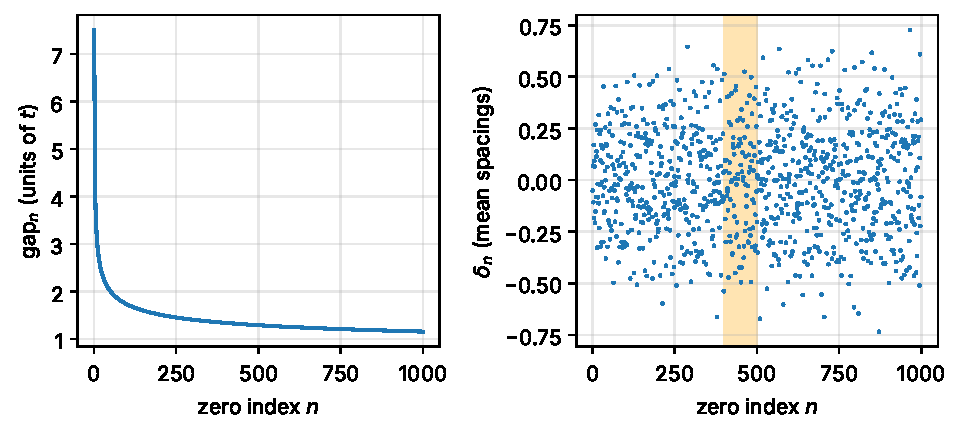
\includegraphics[width=0.85\linewidth]{figs/counting-zeros_fluct.pdf}
\caption{Left: the local mean spacing $\gap_n=2\pi/\log(s_n/2\pi)$ against zero index $n$ for $n\le1000$, in units of $t$; it falls from $7.5$ at $n=1$ to about $1.16$ at $n=1000$. Right: the fluctuations $\delta_n=(t_n-s_n)/\gap_n$ (dimensionless, in mean spacings) for $n\le1000$. The shaded band is the paper's principal holdout, zeros 401--500, over which the rms of $\delta_n$ is $0.263$: the ``null'' error of the paper.}
\label{fig:counting-zeros-fluct}
\end{figure}

\begin{pitfall}
Mind the sign convention. In this chapter $\delta_n=(t_n-s_n)/\gap_n$ is ``truth minus smooth''. The quantity $y_n=n-\tfrac12-\Nsm(t_n)$ used as a fitting target in the paper's Sec.~II~D has the \emph{opposite} sign to first order ($y_n\approx-\delta_n\approx S(t_n)$). The rms is the same either way, but a correlation of $+0.9$ with one becomes $-0.9$ with the other. Always check which convention a formula uses.
\end{pitfall}

\begin{checkpoint}
A prediction misses zero $n$ by $0.2$ in units of $t$. If you move to a height where the mean spacing is half as large, and the miss in $t$ stays $0.2$, what happens to the error in mean spacings?
\checkanswer{It doubles, from $0.2/\gap$ to $0.2/(\gap/2)=0.4/\gap$. The same absolute error is a larger fraction of a spacing where zeros are denser.}
\end{checkpoint}

\begin{keyideas}
\item The fluctuation $\delta_n=(t_n-s_n)/\gap_n$ measures each zero's displacement from its smooth position in local mean spacings.
\item To excellent accuracy, $\delta_n\approx\Nsm(t_n)-(n-\tfrac12)\approx-S(t_n)$, and the unfolded zeros $\Nsm(t_n)$ have unit mean spacing.
\item Errors in mean spacings are comparable across heights; the rms of $\delta_n$ over zeros 401--500 is $0.263$, the paper's null.
\end{keyideas}

%=====================================================================
\section{Paper connection}\label{sec:counting-zeros-paper}

This chapter supplies the yardstick for the entire paper \cite{soniR1}. Here is where each idea appears.

\paragraph{Eq.~(1) and its constant.} The paper's Eq.~(1), $\Nsm(t)=\frac t{2\pi}\log\frac t{2\pi}-\frac t{2\pi}+\frac78$, is introduced in Sec.~II~A as ``the Riemann--von Mangoldt counting function''. You have now derived it: Eq.~\eqref{eq:counting-zeros-NsmS} shows it is $\theta(T)/\pi+1$ with the $1/(48\pi T)$ term dropped, and the $\frac78$ is $-\frac18+1$. The paper does not name the difference $N(t)-\Nsm(t)$; in this book's notation it is $S(t)$, by Eq.~\eqref{eq:counting-zeros-split}, up to the $\order(1/t)$ term. The paper only approximates it, by the prime sum $\Nfl$ of its Eq.~(4).

\paragraph{Smooth zeros and the mean spacing (Sec.~II~A, App.~A step 2).} The paper defines smooth zeros by ``$\Nsm(s_n)=n-\tfrac12$'' and the local mean spacing by ``$\gap_n=ds_n/dn$'', exactly Eqs.~\eqref{eq:counting-zeros-sndef} and \eqref{eq:counting-zeros-gap}. App.~A step 2 says the smooth zeros were found by Brent's method on $\Nsm(t)=n-\tfrac12$ (our first route) and that $\gap$ was computed as \texttt{np.gradient} of the array of smooth zeros, a central finite difference $(s_{n+1}-s_{n-1})/2$ for interior $n$. That agrees with the analytic derivative $2\pi/\log(s_n/2\pi)$ to better than one part in $10^4$ at interior indices such as $n=450$ (checked in the CHECKS script); only at the ends of the array, where \texttt{np.gradient} switches to a one-sided difference, do the two definitions differ appreciably. The companion library \texttt{qmnt.mean\_gap} uses the analytic form.

\paragraph{The Lambert-$W$ asymptotic (Sec.~I~A, paragraph b).} The paper notes that Fran\c ca and LeClair \cite{francaleclair} derived an equation for the $n$-th zero ``whose smooth part is the Lambert-$W$ asymptotic of the counting function''. That smooth part is our Eq.~\eqref{eq:counting-zeros-lambert}: setting $S=0$ in the counting relation and solving for the height gives $s_n$ in closed form.

\paragraph{Every rms in the paper is in mean spacings.} Sec.~II~A states: ``All errors below are quoted in units of the local mean spacing $\gap_n$'', and App.~A repeats: ``All rms values in units of local mean spacing from the smooth zeros of Eq.~(1)''. So every rms in Tables~I--V, and every rms interval quoted in Secs.~III--V (the correlation intervals are pure numbers), is an error measured in units of $\gap_n$ as in Eq.~\eqref{eq:counting-zeros-fluct}. To translate into units of $t$, multiply by the local spacing: near zero 500 (paper's $t_{500}=811.184$, App.~A key anchors) the spacing is $1.293$ (Table~\ref{tab:counting-zeros-gaps}), so the null $0.263$ corresponds to about $0.34$ in $t$.

\paragraph{The null 0.263 (Sec.~II~C, Tables I and V, App.~A).} The paper's baseline prediction is ``no fluctuation'': predict $t_n\approx s_n$. Its error in mean spacings is exactly $\delta_n$, so its rms over zeros 401--500 is the rms of $\delta_n$ there, $0.263$ (App.~A key anchor $0.2631$; Table~V first row). Sec.~II~C explains that the operator null (the unperturbed potential's levels) coincides numerically with this smooth-zero null on 401--500, ``both $0.2631$'', which is why one baseline serves the whole paper. You reproduced this number in Sec.~\ref{sec:counting-zeros-unfold}.

\paragraph{The slow growth of the null (Table V, Sec.~II~C ``Within-height splits'').} The null column of Table~V grows from $0.263$ (401--500) to $0.270$, $0.279$, $0.288$ and $0.296$ (5001--10000). This is the slow growth of the typical size of $S$ described in Sec.~\ref{sec:counting-zeros-S}. The paper calls it a ``covariate shift'' in its within-height-splits paragraph: zeros held out above the training range have slightly larger fluctuations. The nulls of Table~III, $0.23$--$0.27$, are the analogous baseline (the unperturbed potential's error) on other subsets of zeros; the paper reports that this operator null coincides numerically with the rms of $\delta_n$ on the principal holdout 401--500.

\paragraph{Unfolding and Fig.~2.} Sec.~II~A says ``Unfolded spacings of the first $10^4$ zeros show textbook GUE level repulsion (Fig.~2)''. The unfolding is the map $t\mapsto\Nsm(t)$ of Sec.~\ref{sec:counting-zeros-unfold}, which makes the mean spacing 1. The level statistics themselves are Chapter~\ref{ch:level-statistics}.

\paragraph{The oracle and the fitted controls (Sec.~II~D, Eq.~(4)).} The paper's arithmetic oracle predicts zero $n$ by solving $\Nsm(t)+\Nfl(t)=n-\tfrac12$. Compare with the Riemann--von Mangoldt formula at the midpoint of the $n$-th riser, $\Nsm(t_n)+S(t_n)\approx n-\tfrac12$ (Eq.~\eqref{eq:counting-zeros-faces2}): the oracle is this relation (exact up to the $1/(48\pi t_n)$ term) with the unknown $S$ replaced by an explicit approximation $\Nfl$ built from primes (Chapter~\ref{ch:explicit-formula}). The fitted sinusoidal controls of Sec.~II~D train on ``$y_n=n-\tfrac12-\Nsm(t_n)$'', which by Eq.~\eqref{eq:counting-zeros-faces2} is $S(t_n)$ up to $1/(48\pi t_n)$. So everything in the paper's Sec.~IV is, in the language of this chapter, an attempt to predict $S(t)$ at unseen heights.

\paragraph{Discretization errors in mean spacings (Sec.~II~C, App.~A).} The paper's leakage paragraph notes that finite-difference dispersion ``at levels 401--500 on the working grid reaches two mean spacings'', and App.~A records a ``raw-zero null on the uncorrected working grid $2.09$''. Both are in units of $\gap_n$; near zero 450 two mean spacings are about $2.6$ in $t$. Chapter~\ref{ch:finite-differences} explains where these errors come from.

\paragraph{The data and the critical line (Sec.~II~A).} The paper computes $t_1,\dots,t_{1000}$ with \texttt{mpmath} at 20 digits, quoting $t_1=14.134725141734695$ and $t_{1000}=1419.42248094599$. From Table~\ref{tab:counting-zeros-gaps}, $\Nsm(t_{1000})=999.418$, so $\delta_{1000}\approx999.418-999.5=-0.082$: zero 1000 sits $0.08$ spacings below its smooth position. Writing every zero as $\frac12+it_n$ relies on the numerical verification of RH described in Sec.~\ref{sec:counting-zeros-S}.

\paragraph{Overloaded symbols.} In this chapter $N$ is the counting function and $T$ a height. In the paper, $N$ also denotes the number of grid points (Sec.~II~B: ``$N=6000$ at scale 1''), and $T$ also denotes the length of a training window in $t$ (App.~A steps 20 and 23, ``$2\pi/T$'', ``$\pi/T$''); $T$ further labels the second-order tensors $T^{(n)}$ of the paper's Eq.~(5) and the Chebyshev polynomials $T_k$ of its Sec.~II~C. Context always tells you which is meant.

%=====================================================================
\section{Summary}\label{sec:counting-zeros-summary}
% DYK-BEGIN
\begin{didyouknow}{Riemann's Hidden Notes}
Riemann published no numerical work on the zeros, so for decades many assumed his hypothesis was a hunch. In 1932 Carl Ludwig Siegel studied Riemann's unpublished papers in the G\"ottingen library and found a powerful formula for computing zeta on the critical line. Now called the Riemann-Siegel formula, it showed that Riemann had computed zeros himself, and it remains at the core of large-scale zero computations.
\end{didyouknow}
% DYK-END

\begin{itemize}
\item $N(T)$ counts zeros with $0<t_n\le T$; it is a staircase rising by 1 at each (simple) zero (Sec.~\ref{sec:counting-zeros-staircase}).
\item Argument principle: the net change of $\arg f$ around a closed curve, divided by $2\pi$, counts the zeros inside, Eq.~\eqref{eq:counting-zeros-argprinciple} (general theorem taken on trust).
\item Riemann--von Mangoldt formula, Eq.~\eqref{eq:counting-zeros-RvM}: $N(T)=\theta(T)/\pi+1+S(T)$, with $\theta$ of Eq.~\eqref{eq:counting-zeros-thetadef} and $S(T)=\frac1\pi\arg\zeta(\frac12+iT)$, Eq.~\eqref{eq:counting-zeros-Sdef}.
\item Stirling gives $\theta(t)=\frac t2\log\frac t{2\pi}-\frac t2-\frac\pi8+\frac1{48t}+\order(t^{-3})$, Eq.~\eqref{eq:counting-zeros-thetaasym}.
\item Hence $N(T)=\Nsm(T)+S(T)+\frac1{48\pi T}+\order(T^{-3})$ with $\Nsm$ the paper's Eq.~(1), Eqs.~\eqref{eq:counting-zeros-Nsm} and \eqref{eq:counting-zeros-NsmS}; $\frac78=-\frac18+1$.
\item $S(T)$ jumps by $+1$ at zeros and drifts down with slope $-\frac1{2\pi}\log\frac T{2\pi}$ between them, Eq.~\eqref{eq:counting-zeros-Sslope}; $S=\order(\log T)$; typical size of a few tenths at the paper's heights.
\item Smooth zeros: $\Nsm(s_n)=n-\frac12$, Eq.~\eqref{eq:counting-zeros-sndef}, exactly $s_n=2\pi(n-\frac{11}8)/W((n-\frac{11}8)/e)$, Eq.~\eqref{eq:counting-zeros-lambert}.
\item Mean spacing: $\gap_n=\dd s_n/\dd n=2\pi/\log(s_n/2\pi)$, Eq.~\eqref{eq:counting-zeros-gap}.
\item Fluctuation in mean spacings: $\delta_n=(t_n-s_n)/\gap_n\approx\Nsm(t_n)-(n-\frac12)\approx-S(t_n)$, Eqs.~\eqref{eq:counting-zeros-fluct}--\eqref{eq:counting-zeros-faces2}; its rms over zeros 401--500 is the paper's null $0.263$.
\end{itemize}

%=====================================================================
\section{Problems}\label{sec:counting-zeros-problems}

\begin{problemlist}
\prob{1}{Using the ten heights of RE1, Eq.~\eqref{eq:counting-zeros-RE1}, find $N(20)$, $N(35)$ and $N(48.1)$.}

\prob{1}{Evaluate $\Nsm(2\pi)$ and $\Nsm(2\pi e)$ exactly. Compare each with the true count $N$ at the same height ($2\pi e\approx17.08$). What does this tell you about using $\Nsm$ at very low heights?}

\prob{1}{Show from Eq.~\eqref{eq:counting-zeros-Nsm} that $\Nsm'(t)=\frac{1}{2\pi}\log\frac{t}{2\pi}$, showing the product-rule step. Find the mean spacing at $t=2\pi e^2\approx46.43$.}

\prob{1}{Compute the local mean spacing $2\pi/\log(t/2\pi)$ at $t=1000$.}

\prob{1}{A prediction misses a zero near height $t=1000$ by $0.1$ in units of $t$. Express the error in local mean spacings.}

\prob{1}{Use the argument principle to find $\frac{1}{2\pi}\Delta_C\arg(z^3-1)$ when $C$ is (a) the circle $\abs z=2$ and (b) the circle $\abs{z-1}=\frac12$, both traversed counterclockwise.}

\prob{1}{Suppose (contrary to every computation) that $\zeta$ had a double zero at height $t^\ast$. By how much would $N(T)$ and $S(T)$ jump at $T=t^\ast$? Would the number of sign changes of $Z(t)$ near $t^\ast$ change?}

\prob{2}{Verify the Riemann--von Mangoldt formula at $T=30$: compute $\theta(30)$ from Eq.~\eqref{eq:counting-zeros-thetaasym}, then $S(30)$ from Eq.~\eqref{eq:counting-zeros-Sfromcount} using $N(30)=3$. Compare with \texttt{mpmath.backlunds(30)}.}

\prob{2}{Use Eq.~\eqref{eq:counting-zeros-lambert} to compute $s_{100}$ and $\gap_{100}$. Given $t_{100}=236.524230$, find the fluctuation $\delta_{100}$.}

\prob{2}{Show that $\gap_n=2\pi\big/\bigl[1+W\bigl((n-\frac{11}8)/e\bigr)\bigr]$.}

\prob{2}{(Paper.) The paper's Sec.~II~A quotes $t_{1000}=1419.42248094599$. Compute $\Nsm(t_{1000})$, the approximate fluctuation $\delta_{1000}$ using Eq.~\eqref{eq:counting-zeros-faces1}, and the local mean spacing there.}

\prob{2}{(Paper.) The null error on zeros 401--500 is $0.263$ mean spacings (paper Table~V). Using the paper's anchor $t_{500}=811.1843588465$ (App.~A), estimate this error in units of $t$.}

\prob{2}{Using Eq.~\eqref{eq:counting-zeros-Sslope}, find the slope $\dd S/\dd T$ at $T=30$. Over a gap of one local mean spacing, how much does $S$ fall? Comment.}

\prob{2}{Show that $\Nsm$ is decreasing on $(0,2\pi)$ and increasing on $(2\pi,\infty)$, and that its minimum value is $-\frac18$. Explain why this makes the condition $s_n>2\pi$ in Eq.~\eqref{eq:counting-zeros-sndef} necessary for uniqueness.}

\prob{2}{(Paper, computational.) Using \texttt{qmnt}, compute the rms of $\delta_n$ over zeros 401--500, 501--1000 and 1001--2000. Compare with the null column of the paper's Table~V.}

\prob{2}{(Computational.) Using \texttt{qmnt.zeros(1000)} and \texttt{qmnt.fluct}, find the largest $\abs{\delta_n}$ for $n\le1000$ and the index at which it occurs. Is it consistent with the statement that $S$ is ``a few tenths'' at these heights? Explain the difference between a typical value and a maximum.}

\prob{2}{How many zeros do you expect, on average, between heights 1000 and 1001?}

\prob{2}{For $n=1$, evaluate the second-order term $(t_1-s_1)^2/(4\pi s_1)$ in Eq.~\eqref{eq:counting-zeros-faces1} and compare it with the difference between $\Nsm(t_1)-\frac12$ and $\delta_1$.}

\prob{2}{A \emph{Gram point} $g_k$ is defined by $\theta(g_k)=k\pi$. Using Eq.~\eqref{eq:counting-zeros-thetaasym} and Newton's method, find $g_0$ (the solution with $g_0>2\pi$). Check with \texttt{mpmath.grampoint(0)}.}

\prob{2}{(Paper.) The paper's Sec.~II~C says that finite-difference dispersion at levels 401--500 on the working grid ``reaches two mean spacings''. Using Table~\ref{tab:counting-zeros-gaps}, estimate this in units of energy (which equal units of $t$ in the paper's conventions).}

\prob{2}{(Computational.) Show that the mean of the unfolded spacings $x_{n+1}-x_n$, $n=1,\dots,N-1$, equals $(x_N-x_1)/(N-1)$. Compute it for $N=10$ from RE1, and then with \texttt{qmnt} for $N=1000$.}

\prob{2}{(Paper.) The fitted controls of the paper's Sec.~II~D train on $y_n=n-\frac12-\Nsm(t_n)$. Show that $y_n\approx S(t_n)\approx-\delta_n$, compute $y_1$, and explain why a model that predicts $y_n$ well automatically predicts the zeros well.}

\prob{3}{(Computational.) Using \texttt{mpmath} with at least 30 digits, compute $t^3\bigl[\theta(t)-\frac t2\log\frac t{2\pi}+\frac t2+\frac\pi8-\frac{1}{48t}\bigr]$ at $t=50$ and $t=200$, and compare with $7/5760$.}

\prob{3}{Fill in the symmetry argument of Sec.~\ref{sec:counting-zeros-rvm} in detail: parametrize $P$ and $P'$ explicitly, and show that $\arg\xi$ at the point of $P'$ corresponding to parameter value $\tau$ equals $-\arg\xi$ at the mirror point of $P$, and hence that $\Delta_{P'}\arg\xi=\Delta_P\arg\xi$.}

\prob{3}{Explain, step by step, why the following procedure proves that all zeros with $0<t<T$ lie on the critical line and are simple: (i) find $k$ sign changes of $Z(t)$ in $(0,T)$; (ii) establish that $N(T)=k$ exactly. Which step needs $S(T)$, and why can't one simply evaluate $\Nsm(T)$ and round?}

\prob{2}{Compute $\xi(2)$ exactly from Eq.~\eqref{eq:counting-zeros-xi} using $\zeta(2)=\pi^2/6$ and $\Gamma(1)=1$. Then, using \texttt{mpmath} (\texttt{mp.zeta}, \texttt{mp.gamma}), evaluate the right side of Eq.~\eqref{eq:counting-zeros-xi} at $s=-1$ and confirm that $\xi(-1)=\xi(2)$, as the functional equation requires. Which two factors are negative at $s=-1$?}

\prob{3}{(Paper, computational.) The paper cites the Lambert-$W$ asymptotic of Fran\c ca and LeClair (Sec.~I~A, paragraph b). Compute $s_n$ for $n=1,\dots,1000$ both from Eq.~\eqref{eq:counting-zeros-lambert} and with \texttt{qmnt.smooth\_zeros}, and find the largest absolute difference. Explain why the two must agree to within root-finding tolerance.}

\prob{3}{Selberg's theorem says the mean square of $S$ grows like $\frac{1}{2\pi^2}\log\log T$. Compute $\sqrt{\log\log T/(2\pi^2)}$ at $T=10^3$ and $T=10^4$ and the ratio of the two. Compare with the ratio of the paper's nulls $0.296/0.263$ (Table~V). Discuss why you should not expect close agreement (consider lower-order terms, and the difference between $S$ at all heights and $S$ at the zeros).}
\end{problemlist}

%=====================================================================
\section{Answers to selected problems}\label{sec:counting-zeros-answers}

\textbf{1.} $t_1=14.13<20<t_2=21.02$, so $N(20)=1$. $t_5=32.94<35<t_6=37.59$, so $N(35)=5$. $t_9=48.005<48.1<t_{10}=49.77$, so $N(48.1)=9$.

\textbf{2.} $\Nsm(2\pi)=1\cdot\log1-1+\frac78=-\frac18$. $\Nsm(2\pi e)=e\log e-e+\frac78=\frac78$. True counts: $N(2\pi)=0$ and $N(2\pi e)=N(17.08)=1$. At these low heights $\Nsm$ is off by $\frac18$ of a zero and is even negative at $2\pi$; it is an asymptotic formula, and its relative accuracy improves with height. (Its absolute error, $S$, does not shrink.)

\textbf{3.} $\frac{\dd}{\dd t}\bigl[\frac t{2\pi}\log\frac t{2\pi}\bigr]=\frac1{2\pi}\log\frac t{2\pi}+\frac t{2\pi}\cdot\frac1t$ by the product rule (the derivative of $\log(t/2\pi)$ is $1/t$). Subtracting the derivative $\frac1{2\pi}$ of $\frac t{2\pi}$ leaves $\frac1{2\pi}\log\frac t{2\pi}$. At $t=2\pi e^2$, $\log(t/2\pi)=2$, so the mean spacing is $2\pi/2=\pi\approx3.14$.

\textbf{4.} $\log(1000/2\pi)=6.907755-1.837877=5.069878$; spacing $6.283185/5.069878=1.239$.

\textbf{5.} $0.1/1.239=0.0807$ mean spacings.

\textbf{6.} The zeros are $1$, $e^{2\pi i/3}$ and $e^{-2\pi i/3}$, all of modulus 1. (a) All three lie inside $\abs z=2$: answer 3. (b) The distance from $1$ to $e^{\pm2\pi i/3}=-\frac12\pm\frac{\sqrt3}2i$ is $\sqrt{(3/2)^2+3/4}=\sqrt3>\frac12$, so only $z=1$ is inside: answer 1.

\textbf{7.} $N$ would jump by 2 (zeros are counted with multiplicity), and since $\theta$ is continuous, $S$ would also jump by 2. Near a double zero $Z(t)$ behaves like a constant times $(t-t^\ast)^2$ and does not change sign; a sign-change count would see no zero there at all, while $N(T)$ would count two. This mismatch is exactly what the procedure of Problem~25 detects.

\textbf{9.} $x_{100}=98.625/e=36.282110$; solving $we^w=x_{100}$ gives $W=2.625901$. Then $s_{100}=2\pi\times98.625/2.625901=619.679151/2.625901=235.987$; $\gap_{100}=2\pi/3.625901=1.733$; $\delta_{100}=(236.524230-235.987266)/1.733=0.536964/1.733=+0.310$. Zero 100 sits about a third of a spacing above its smooth position.

\textbf{11.} $u=1419.422481/2\pi=225.908136$, $\log u=5.420128$; $\Nsm(t_{1000})=225.908136\times4.420128+0.875=998.542976+0.875=999.418$. By Eq.~\eqref{eq:counting-zeros-faces1}, $\delta_{1000}\approx999.418-999.5=-0.082$ (the second-order term is about $2\times10^{-6}$). Spacing: $2\pi/5.420128=1.159$.

\textbf{13.} $\dd S/\dd T=-\frac{1}{2\pi}\log\frac{30}{2\pi}+\frac{1}{48\pi\cdot900}=-\frac{1.563320}{6.283185}+0.000007=-0.249$. Over one local mean spacing $\gap=1/\Nsm'(30)$, $S$ falls by $\Nsm'(30)\times\gap=1$ (to the accuracy of the tiny $1/(48\pi T^2)$ term). This is why perfectly evenly spaced zeros would leave $S$ oscillating between fixed limits: each jump of $+1$ is exactly undone by the drift across one mean spacing.

\textbf{15.} The rms values are $0.263$, $0.270$, $0.279$, matching the paper's Table~V nulls for 401--500, 501--1000 and 1001--2000. The paper computes $\gap_n$ by \texttt{np.gradient}, \texttt{qmnt} analytically; the difference is invisible at three decimals.

\textbf{17.} The expected number is $\Nsm(1001)-\Nsm(1000)=\int_{1000}^{1001}\Nsm'(t)\,\dd t\approx\Nsm'(1000.5)=\frac{1}{2\pi}\log\frac{1000.5}{2\pi}=\frac{5.070378}{6.283185}=0.807$. (The midpoint rule is accurate to about $10^{-8}$ here because $\Nsm''$ is tiny.)

\textbf{19.} Solve $f(g)=\frac g2\log\frac g{2\pi}-\frac g2-\frac\pi8+\frac1{48g}=0$ with $f'(g)\approx\frac12\log\frac g{2\pi}$. Starting from $g=17.8$, $f(17.8)\approx-0.0238$ and $f'(17.8)\approx0.5207$, so the first step gives $17.8\,+\,0.0238/0.5207\approx17.8457$. A second step changes this only in the fifth decimal, giving $g_0=17.8456$. Because $f$ is increasing and convex there ($f''\approx1/(2g)>0$), a Newton step started to the left of the root lands slightly to its right, by about $6\times10^{-5}$ here. \texttt{mpmath.grampoint(0)} gives $17.8456$ as well.

\textbf{21.} The sum $\sum_{n=1}^{N-1}(x_{n+1}-x_n)$ telescopes to $x_N-x_1$, so the mean is $(x_N-x_1)/(N-1)$. For $N=10$: $(9.348203-0.449278)/9=0.989$ (Sample Problem in Sec.~\ref{sec:counting-zeros-unfold}). For $N=1000$ the same formula with $x_{1000}=\Nsm(t_{1000})=999.418$ gives $(999.418-0.449)/999=0.99997$; the departure from 1 is $(\delta_{1000}-\delta_1)/999$, which shrinks as $N$ grows because the $\delta_n$ do not grow appreciably.

\textbf{23.} At $t=50$ the bracket times $t^3$ is $0.001215$, and at $t=200$ it is closer still to $7/5760=0.0012153$. The next term in the expansion is of order $t^{-5}$, so $t^3\times$(remainder) approaches $7/5760$ with a correction of order $t^{-2}$, about $10^{-7}$ at $t=50$.

\textbf{25.} Each sign change of the real function $Z(t)$ in $(0,T)$ requires a zero of $\zeta(\frac12+it)$ of odd multiplicity on the critical line, so there are at least $k$ zeros on the line, counted with multiplicity. If $N(T)=k$ exactly, the total number of zeros in the strip below $T$ (on or off the line, with multiplicity) is also $k$. So there is no zero left over to lie off the line, and no zero can be multiple (a multiple zero would contribute more than 1 to $N$ while producing at most one sign change). Step (ii) needs $S(T)$, because $N(T)=\theta(T)/\pi+1+S(T)$. Rounding $\Nsm(T)$ fails because $S(T)$ is of order a few tenths and can exceed $\frac12$ in magnitude (for example $S(50)=0.577$), so the nearest integer to $\Nsm(T)$ can be wrong. Turing's method supplies a rigorous way to pin down the integer.

\textbf{27.} The largest difference is at the level of the root finder's tolerance (about $10^{-9}$ or smaller). Both methods solve the same equation $\Nsm(s)=n-\frac12$ on the branch $s>2\pi$, where the solution is unique (Problem~14); Eq.~\eqref{eq:counting-zeros-lambert} is the exact solution, so any difference is numerical error in the root finder or in the evaluation of $W$.
